% Copyright 2020, 2021  Ed Bueler

\documentclass[10pt,dvipsnames,usepdftitle=false,
hyperref={pdftitle = {Finite volume methods},
    pdfauthor = {Ed Bueler}}]{beamer}

\mode<presentation>{
  \usetheme{Madrid}
  \usecolortheme{beaver}
  \setbeamercovered{transparent}  
  \setbeamerfont{frametitle}{size=\large}
}

\setbeamercolor*{block title}{bg=red!10}
\setbeamercolor*{block body}{bg=red!5}

\usepackage[english]{babel}
\usepackage[latin1]{inputenc}
\usepackage{times}
\usepackage[T1]{fontenc}
% Or whatever. Note that the encoding and the font should match. If T1
% does not look nice, try deleting the line with the fontenc.

\usepackage{empheq}
\usepackage{xspace}
\usepackage{verbatim,fancyvrb}

\usepackage{tikz}
\usetikzlibrary{shapes,arrows.meta,decorations.markings,decorations.pathreplacing,fadings,positioning}

\usepackage{cancel}

% If you wish to uncover everything in a step-wise fashion, uncomment
% the following command: 
%\beamerdefaultoverlayspecification{<+->}

\newcommand{\ba}{\mathbf{a}}
\newcommand{\bb}{\mathbf{b}}
\newcommand{\bc}{\mathbf{c}}
\newcommand{\bbf}{\mathbf{f}}
\newcommand{\bg}{\mathbf{g}}
\newcommand{\bn}{\mathbf{n}}
\newcommand{\bq}{\mathbf{q}}
\newcommand{\br}{\mathbf{r}}
\newcommand{\bx}{\mathbf{x}}
\newcommand{\by}{\mathbf{y}}
\newcommand{\bv}{\mathbf{v}}
\newcommand{\bu}{\mathbf{u}}
\newcommand{\bw}{\mathbf{w}}

\newcommand{\bF}{\mathbf{F}}
\newcommand{\bG}{\mathbf{G}}
\newcommand{\bQ}{\mathbf{Q}}

\newcommand{\grad}{\nabla}
\newcommand{\Div}{\nabla\cdot}
\newcommand{\minmod}{\operatorname{minmod}}

\newcommand{\CC}{\mathbb{C}}
\newcommand{\RR}{\mathbb{R}}

\newcommand{\ddt}[1]{\ensuremath{\frac{\partial #1}{\partial t}}}
\newcommand{\ddx}[1]{\ensuremath{\frac{\partial #1}{\partial x}}}
\newcommand{\Matlab}{\textsc{Matlab}\xspace}
\newcommand{\Octave}{\textsc{Octave}\xspace}
\newcommand{\eps}{\epsilon}

\newcommand{\ip}[2]{\left<#1,#2\right>}

\newcommand{\half}{\tfrac{1}{2}}

\newcommand{\xiphalf}{{x_{i+\frac{1}{2}}}}
\newcommand{\ximhalf}{{x_{i-\frac{1}{2}}}}
\newcommand{\Fiphalf}{{F_{i+\frac{1}{2}}}}
\newcommand{\Fimhalf}{{F_{i-\frac{1}{2}}}}
\newcommand{\Fiphalfn}{{F^n_{i+\frac{1}{2}}}}
\newcommand{\Fimhalfn}{{F^n_{i-\frac{1}{2}}}}

\newcommand{\trefcolumn}[1]{\begin{bmatrix} \phantom{x} \\ #1 \\ \phantom{x} \end{bmatrix}}
\newcommand{\trefmatrixtwo}[2]{\left[\begin{array}{c|c|c} & & \\ #1 & \dots & #2 \\ & & \end{array}\right]}
\newcommand{\trefmatrixthree}[3]{\left[\begin{array}{c|c|c|c} & & & \\ #1 & #2 & \dots & #3 \\ & & & \end{array}\right]}
\newcommand{\trefmatrixgroups}[4]{\left[\begin{array}{c|c|c|c|c|c} & & & & & \\ #1 & \dots & #2 & #3 & \dots & #4 \\ & & & & & \end{array}\right]}

\newcommand{\blocktwo}[4]{\left[\begin{array}{c|c} #1 & #2 \\ \hline #3 & #4 \end{array}\right]}

\newcommand{\bqed}{{\color{blue}\qed}}
\newcommand{\ds}{\displaystyle}

\newcommand\mynum[1]{{\renewcommand{\insertenumlabel}{#1}%
      \usebeamertemplate{enumerate item} \,}}


\title[Finite volume methods]{Finite volume methods for \\ advection equations and hyperbolic systems}

\subtitle{version 3, April 2021}
%version 2: \date{June 2020}

\author{Ed Bueler, UAF}

\date{}

\titlegraphic{\vspace{-10mm} 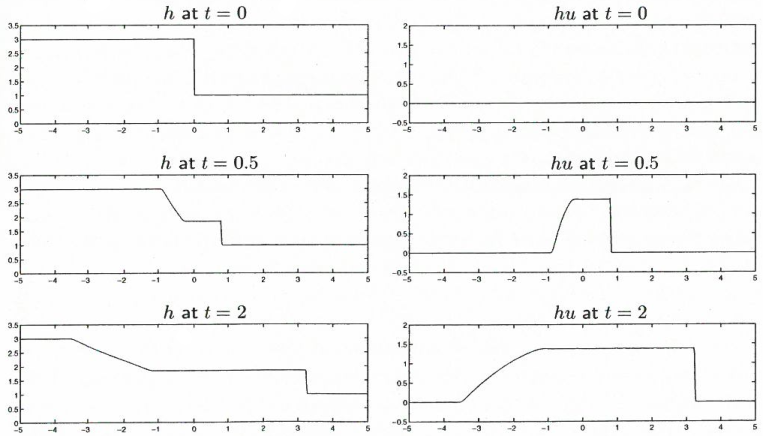
\includegraphics[width=0.5\textwidth]{figs/leveque13p4}}

%\institute[UAF]{University of Alaska Fairbanks}

% this nonsense needed to start section counter at 0; see
% https://tex.stackexchange.com/questions/170222/change-the-numbering-in-beamers-table-of-content
\makeatletter
\patchcmd{\beamer@sectionintoc}
  {\ifnum\beamer@tempcount>0}
  {\ifnum\beamer@tempcount>-1}
  {}
  {}
\beamer@tocsectionnumber=-1
\makeatother


\begin{document}
\beamertemplatenavigationsymbolsempty

\begin{frame}
  \maketitle
\end{frame}

\begin{frame}
  \frametitle{Outline}
  \tableofcontents[hideallsubsections]
\end{frame}


\section{overview and scope}

\begin{frame}[fragile]
\frametitle{overview}

\begin{itemize}
\item numerical solutions of systems of first-order, time-dependent PDEs
\item hyperbolic PDEs:

\bigskip
\begin{center}
\begin{tikzpicture}[scale=0.85,
                    >={Latex[length=2mm]},
  eqn/.style={
     rectangle,draw,fill=white,align=center,line width=0.6pt,minimum width=15mm}]

%center
\draw[line width=1pt] (0,0)     node[eqn] (scalaradvect)  {\mynum{1} scalar advection \\ {\Large \strut} $q_t + a q_x=0$};
\draw[line width=1pt] (3,-1.7)     node[eqn] (scalartwod)  {\mynum{5} scalar advection in 2D \\ {\Large \strut} $q_t + (u q)_x + (v q)_y=0$};
\draw[line width=1pt] (-2,-1.7)    node[eqn] (linearsystem)  {\mynum{2} linear systems \\ {\Large \strut} $\bq_t + A\, \bq_x=0$};
\draw[line width=1pt] (-2,-3.55)    node[eqn] (generalsystem)  {\mynum{4} conservation-law systems \\ {\Large \strut} $\bq_t + \bF(t,x,\bq)_x=\bg(t,x,\bq)$};

\path[-Latex]
   ([xshift=-2em]scalaradvect.south) edge node {} (linearsystem)
   ([xshift=2em]scalaradvect.south) edge node {} (scalartwod)
   (linearsystem.south) edge node {} (generalsystem);
\end{tikzpicture}

\end{center}
\item finite volume (FV) discretizations
    \begin{itemize}
    \item[$\circ$] a genuine introduction to FV methods
    \end{itemize}
\item section \mynum{3} is about ``high-resolution'' flux discretizations
\end{itemize}
\end{frame}


\begin{frame}{references, big and small}
\begin{itemize}
\item {\large \alert{R.~J.~LeVeque, \emph{Finite Volume Methods for Hyperbolic Problems}, Cambridge University Press, 2002}}

\medskip
%\item K.~W.~Morton and D.~F.~Mayers, \emph{Numerical Solutions of Partial Differential Equations: An Introduction}, Cambridge University Press, 2nd ed., 2005
\item W.~Hundsdorfer and J.~G.~Verwer, \emph{Numerical Solution of Time-Dependent Advection-Diffusion-Reaction Equations}, Springer, 2003
\item E.~Bueler, \emph{PETSc for Partial Differential Equations}, SIAM Press, 2020
\end{itemize}

\bigskip

\begin{center}
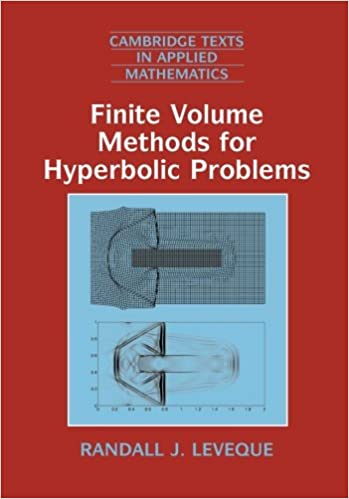
\includegraphics[height=36mm]{figs/covers/leveque} \qquad 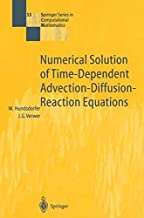
\includegraphics[height=26mm]{figs/covers/hv} \qquad 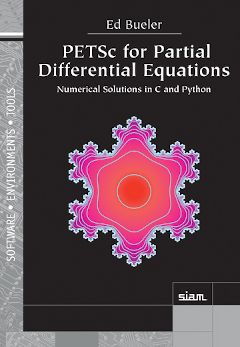
\includegraphics[height=26mm]{figs/covers/bueler}
\end{center}
\end{frame}


\begin{frame}{visual example 1: merely a numerical solution}

\begin{itemize}
\item before getting to numerical solutions, two show-and-tell movies
\item consider advection equation for scalar density $q(t,x)$:
    $$q_t + a \, q_x = 0$$
with speed $a=1$, initial condition $q(0,x)$ known, and periodic boundary conditions on $0\le x \le 1$
\item movie of numerical solution for $0\le t \le 1$
    \begin{itemize}
    \item[$\circ$] initial shape is transported rightward, from initial position back to same position
    \end{itemize}
\end{itemize}

\vspace{10mm}
\begin{center}
\alert{SHOW ADVECTION MOVIE}
\end{center}
\vspace{10mm}

% cd p4pdes-next/c/riemann/
% make riemann
% ./riemann -problem advection -da_grid_x 200 -limiter minmod -ts_monitor_solution binary:q.dat -ts_monitor binary:t.dat
% make petscPyScripts
% mkdir advection
% ./plotTS.py -mx 200 -ylabel "q" -ax 0.0 -bx 1.0 -cellcentered t.dat q.dat -oroot advection/bar
% cd advection
% eog bar*.png
\end{frame}


\begin{frame}{visual example 1: numerical \emph{and exact} solutions}

\begin{itemize}
\item was it clear what the movie showed?
\item figures below are better: they show numerical and exact solutions
\end{itemize}

\bigskip
\hfill \mbox{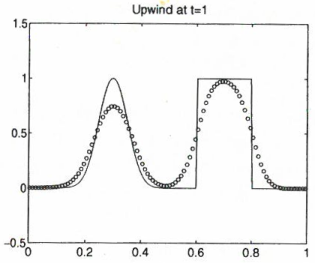
\includegraphics[width=0.48\textwidth]{figs/leveque6p1upwind} \, 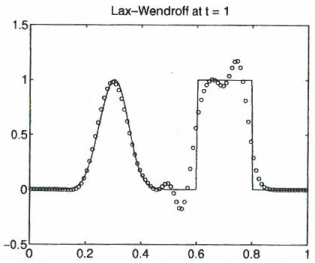
\includegraphics[width=0.48\textwidth]{figs/leveque6p1lw}}
\end{frame}


\begin{frame}{visual example 2: merely a numerical solution}

\begin{itemize}
\item shallow water equations:

\vspace{-11.5mm}
\begin{align*}
\hspace{60mm} h_t + (hu)_x &= 0 \\
(hu)_t + \left(h u^2 + \frac{g}{2} h^2\right)_x &= 0
\end{align*}

\vspace{-5mm}
    \begin{itemize}
    \item[$\circ$] coupled
    \item[$\circ$] hyperbolic
    \item[$\circ$] nonlinear
    \end{itemize}
\item suppose initial condition is a ``hump'' on $x \in [-5,5]$
    \begin{itemize}
    \item[$\circ$] $h(0,x)=a e^{-bx^2}$, $u(0,x)=0$
    \item[$\circ$] vertical displacement in the center of the domain
    \item[$\circ$] simplest model for a tsunami generated in middle of ocean
    \end{itemize}
\item movie of numerical solution for $0 \le t \le 3$

\vspace{10mm}
\begin{center}
\alert{SHOW SHALLOW WATER ``HUMP'' MOVIE}
\end{center}

\vspace{10mm}

% ./riemann -problem swater -initial hump -da_grid_x 1000 -limiter minmod -ts_monitor binary:t.dat -ts_monitor_solution binary:q.dat
% mkdir swater
% ./plotTS.py -mx 1000 -ylabel "h (height)" -ax -5.0 -bx 5.0 -dof 2 -c 0 -cellcentered t.dat q.dat -oroot swater/height
% ./plotTS.py -mx 1000 -ylabel "hu (flux)" -ax -5.0 -bx 5.0 -dof 2 -c 1 -cellcentered t.dat q.dat -oroot swater/flux
% cd swater
% eog height*.png
% eog flux*.png
\end{itemize}
\end{frame}


\begin{frame}{multiple roles for exact solutions}

\begin{itemize}
\item generally, exact solutions are rare but valuable
\item in these slides, exact solutions have two roles:
  \begin{enumerate}
  \item for \emph{verifying} simulations
      \begin{itemize}
      \item[$\circ$] measure norm of difference between exact and numerical solutions
      \item[$\circ$] precise ``mathematical engineering'' of numerical solvers
      \end{itemize}
  \item as \emph{``Riemann solvers''} for hyperbolic systems
      \begin{itemize}
      \item[$\circ$] used locally in constructing the numerical scheme
      \item[$\circ$] solutions for discontinuous initial conditions
      \item[$\circ$] explaining this mystery is a major purpose of my talk!
      \end{itemize}
  \end{enumerate}
\end{itemize}
\end{frame}


\begin{frame}[fragile]

\frametitle{my context: high performance PDEs}

\begin{itemize}
\item I am interested in high performance solutions of PDEs
\item all examples in these slides use fast, but less-elegant, C code
    \begin{itemize}
    \item[$\circ$] compared to Matlab
    \end{itemize}
\item \dots calling the Portable Extensible Toolkit for Scientific computing:

    \begin{center}
    \href{https://www.mcs.anl.gov/petsc/}{\texttt{www.mcs.anl.gov/petsc/}}
    \end{center}

    \begin{itemize}
    \item[$\circ$] a mathematical library for high-performance computing
    \item[$\circ$] by DOE's Argonne National Lab \dots who also brought you MPI
    \end{itemize}
\item the run which generated the previous shallow water movie, with $1000\times 361$ (space$\times$time) grid, completed in 0.3 seconds
% using linux-c-opt:
% timer ./riemann -problem swater -initial hump -da_grid_x 1000 -limiter minmod

\item speed is more critical for problems with 2D and 3D space
    \begin{itemize}
    \item[$\circ$] parallelizability also important there
    \end{itemize}
\end{itemize}
\end{frame}


\begin{frame}{please ask questions}

\begin{itemize}
\item the rest of the talk is about the math not the movies
    \begin{itemize}
    \item[$\circ$] but with many figures to explain concepts
    \end{itemize}
\item \alert{PLEASE} ask lots of questions, about any topic here at all
    \begin{itemize}
    \item[$\circ$] slowing me down is a \emph{good}\, thing!
    \item[$\circ$] I'll try to watch the zoom chat, too
    \end{itemize}
\item feel free to email after the talk, or into the indefinite future:
    \begin{itemize}
    \item[$\circ$] \texttt{elbueler\@@alaska.edu}
    %\item[$\circ$] I might be able to help with numerical questions (but not 615 homework)
    \end{itemize}
\end{itemize}
\end{frame}


\AtBeginSection[]
{
  \begin{frame}<beamer>
    \frametitle{Outline}
    \tableofcontents[currentsection,hideallsubsections]
  \end{frame}
}

\section{scalar advection equation}

\begin{frame}{one-way advection}

\begin{itemize}
\item next few slides should be an easy review
\item consider the \emph{scalar advection PDE} for $q(t,x)$:
    $$q_t + a q_x=0$$

\item if $a$ is constant and we have a smooth initial condition $q(t,0)=f(x)$ then the solution is
    $$q(t,x) = f(x-at),$$
\emph{because}, by the chain rule
\begin{gather*}
q_t + a q_x = -a f'(x-at) + a f'(x-at) = 0
\end{gather*}
\item the solution $q(t,x)=f(x-at)$ is a ``movie'': the graph of $f(x)$ is translated distance by $at$, to the right, in time $t$
    \begin{itemize}
    \item[$\circ$] even if $a$ and/or $t$ are negative
    \item[$\circ$] $a$ is the speed of the motion
    \end{itemize}
\end{itemize}
\end{frame}


\begin{frame}{solution by characteristics}

\begin{itemize}
\item but what about with variable speed $a(t,x)$?
    $$q_t + a(t,x) q_x=0, \qquad q(0,x) = f(x)$$
\item we need the idea of a \emph{characteristic curve} (ODE):
    $$\ds \frac{d\xi}{ds} = a(s,\xi(s)) \hspace{50mm}$$

\vspace{-10mm}

\hfill 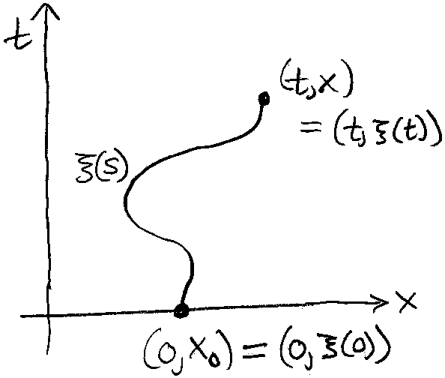
\includegraphics[width=0.32\textwidth]{figs/characteristicsketch}

\vspace{-20mm}
\item for a solution $q(t,x)$, we calculate $\left[\xi'=\tfrac{d\xi}{ds}\right]$
\begin{align*}
\Big(q(s,\xi(s))\Big)' &= q_t(s,\xi(s)) + q_x(s,\xi(s)) \xi'(s) \hspace{40mm} \\
                          &= q_t(s,\xi(s)) + q_x(s,\xi(s)) a(s,\xi(s)) \\
                          &= 0,
\end{align*}
\item conclude: $q(t,\xi(t)) = q(0,\xi(0))$
\item \emph{solution by characteristics}: $q(t,x)$ has the same value as $f(x_0)$ if $\xi(s)$ is a characteristic curve that ends at $(t,x)$ and starts at $(0,x_0)$
\end{itemize}
\end{frame}


\begin{frame}{solution by characteristics 2}

\begin{itemize}
\item the method can be extended to the nonlinear equation
     $$q_t + a(t,x) q_x = g(t,x,q), \qquad q(0,x) = f(x)$$

    \begin{itemize}
    \item[$\circ$] $a$ is the speed of the characteristic curve
    \item[$\circ$] $g$ is the \emph{source term}
    \item[$\circ$] \emph{idea}: the solution $q$ changes at rate $g$ along the characteristic
    \item[$\circ$] if $g=0$ then $q$ is constant along the characteristic
    \end{itemize}
\item now we have a pair of ODEs to solve:
\begin{align*}
\xi'(s) &= a(s,\xi(s)) \\
\omega'(s) &= g(s,\xi(s),\omega(s))
\end{align*}
\item \emph{solution by characteristics}:
    \begin{itemize}
    \item[i)] from 1st ODE, find characteristic $\xi(s)$ through $(0,x_0)$ and $(t,x)$
    \item[ii)] solve 2nd ODE with initial condition $\omega(0)=f(x_0)$
    \item[iii)] then $q(t,x) = \omega(t)$
    \end{itemize}
\item \alert{main idea} about advection PDEs:

\begin{center}
information travels along the characteristics
\end{center}
\end{itemize}
\end{frame}


\begin{frame}{upwind scheme for one-way advection}

\begin{itemize}
\item we may apply the \emph{upwind} scheme to $q_t + aq_x=0$ (case $a>0$):
    $$\frac{Q_i^{n+1} - Q_i^n}{\Delta t} + a \frac{Q_i^n - Q_{i-1}^n}{\Delta x} = 0$$
\item equivalently, solve for the new value at $t_{n+1}$:
\begin{align*}
Q_i^{n+1} &= \frac{a\Delta t}{\Delta x} Q_{i-1}^n + \left(1 - \frac{a\Delta t}{\Delta x}\right) Q_i^n = \ell(x_i-a\Delta t)
\end{align*}
where $\ell(x)$ linearly interpolates

\noindent between $(x_{i-1},Q_{i-1}^n)$ and $(x_i,Q_i^n)$

\vspace{-9mm}
\hfill 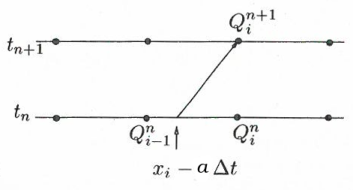
\includegraphics[width=0.45\textwidth]{figs/leveque4p4a}

\vspace{-7mm}
\item interpolate $\ell$ where the characteristic

\noindent through $(x_i,Q_i^{n+1})$ hits the $t_n$ line

\item except we must require \emph{interpolation} instead of extrapolation: $\ds \frac{|a|\Delta t}{\Delta x} \le 1$
\end{itemize}
\end{frame}


\begin{frame}{upwind and Lax-Wendroff schemes}

\begin{itemize}
\item while upwind uses linear interpolation using two points, \dots
\item the \emph{Lax-Wendroff} scheme uses quadratic interpolation with three points
\item formulas: if $\nu = a\Delta t/\Delta x$ then
\begin{align*}
Q_i^{n+1} &= \nu Q_{i-1}^n + \left(1 - \nu\right) Q_i^n &&\text{upwind} \\
Q_i^{n+1} &= \tfrac{1}{2} \nu (1+\nu) Q_{i-1}^n + \left(1 - \nu^2\right) Q_i^n + \tfrac{1}{2} \nu (1-\nu) Q_{i+1}^n &&\text{LW}
\end{align*}

\begin{center}
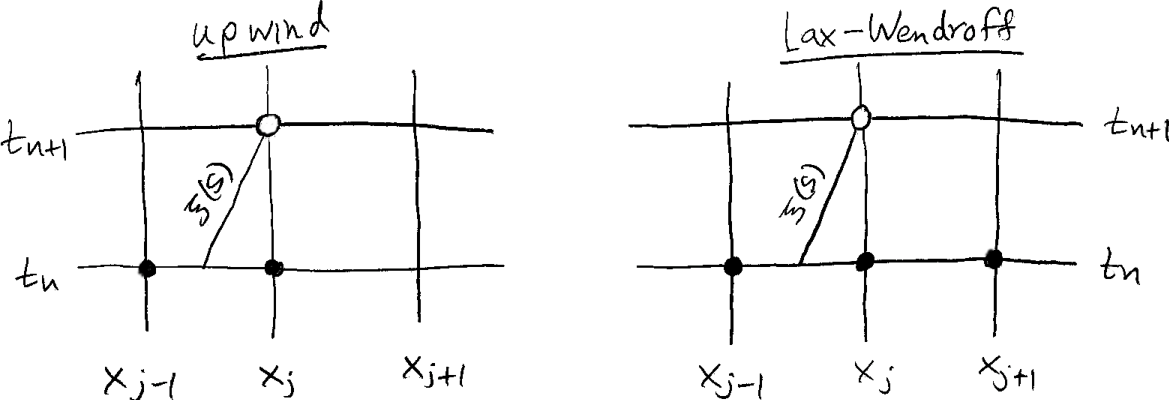
\includegraphics[width=0.95\textwidth]{figs/stencilssketch}
\end{center}
\end{itemize}
\end{frame}


\begin{frame}{four derivations of Lax-Wendroff}

\begin{itemize}
\item by the way \dots
\item can you describe multiple interpretations of Lax-Wendroff?
    \begin{enumerate}
    \item<1-4> quadratic interpolation above
    \item<2-4> \only<2-4>{use spatial difference on $O(\Delta t^2)$ term in Taylor series}
    \item<3-4> \only<3-4>{half steps of Lax-Friedrichs followed by leap-frog}
    \item<4> \only<4>{\emph{revealed later in this talk}}
    \end{enumerate}
\end{itemize}
\end{frame}


\begin{frame}{stability}

\begin{itemize}
\item in a very early paper, Courant, Friedrichs, and Lewy gave a criterion for stability of numerical methods on hyperbolic PDEs
\item \alert{CFL criterion:} the characteristic through the new location $(t_{n+1},x_i)$ must be in the numerical domain of dependence of the scheme at $t_n$, i.e.
    $$\nu_{CFL} = \frac{|a|\Delta t}{\Delta x} \le 1 \qquad \iff \qquad \Delta t \le \frac{\Delta x}{|a|}$$

\item we need CFL so that upwind and Lax-Wendroff formulas are \emph{interpolations} not \emph{extrapolations}
    \begin{itemize}
    \item[$\circ$] the errors from extrapolation would propagate forward as exponential growth, i.e.~\emph{unstably}
    \end{itemize}
\item CFL is a \emph{necessary} condition for stability (and thus for convergence)
\item CFL applies to any finite difference, finite volume, or finite element scheme for a hyperbolic PDE
\end{itemize}
\end{frame}


\begin{frame}{results}

\begin{itemize}
\item suppose same problem as in earlier movie:

$q_t+a q_x=0$, $a=1$, $0\le x\le 1$, and periodic boundary conditions

\medskip
\hfill 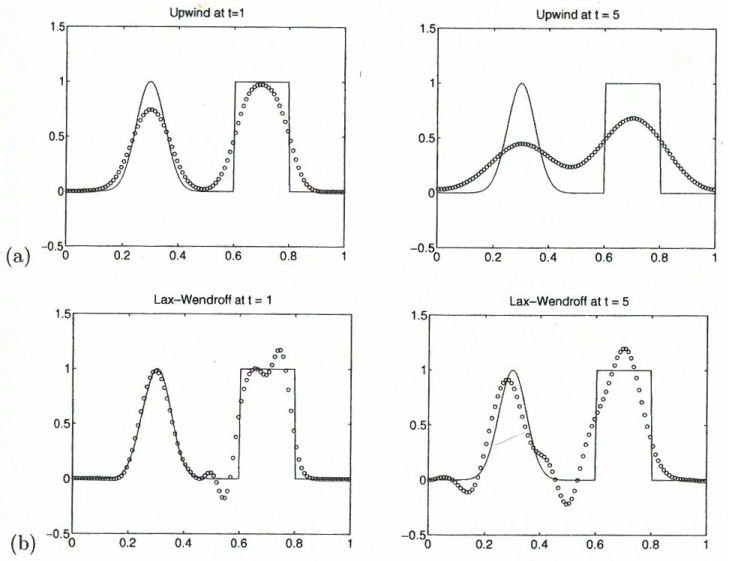
\includegraphics[width=0.72\textwidth]{figs/leveque6p1}

\vspace{-25mm}

\emph{issues:}

\alert{{\footnotesize oversmoothing}

{\footnotesize spurious oscillation}

{\footnotesize loss of original bounds}}
\end{itemize}
\end{frame}


\begin{frame}{how to do better? \dots the history}

\begin{itemize}
\item upwind and Lax-Wendroff methods were obvious technology by $\sim$1960
\item but the results suffered from three diseases:
    \begin{itemize}
    \item[$\circ$] \alert{oversmoothing} (upwind)
    \item[$\circ$] \alert{spurious oscillation} (Lax-Wendroff)
    \item[$\circ$] \alert{loss of original solution bounds} (Lax-Wendroff)
    \end{itemize}

\vspace{-15mm}

\hfill 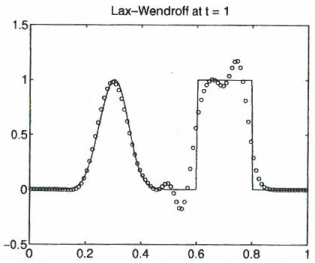
\includegraphics[width=0.3\textwidth]{figs/leveque6p1lw}

\bigskip
\item in 1960--90s these diseases were mostly fixed \dots how?:
    \begin{itemize}
    \item[$\circ$] reading Godunov (1959)
    \item[$\circ$] new ``finite volume'' thinking
    \item[$\circ$] new ``Riemann solver'' interpretation of the upwind method
    \item[$\circ$] new ``slope-limiting'' or ``flux-limiting'' to avoid oscillations
    \end{itemize}

\item this talk: make sense of these 1990s buzzwords!
\end{itemize}
\end{frame}


%\begin{frame}{a \Matlab code to play with}
%\begin{itemize}
%\item mostly I have been playing with PETSc, but \dots
%\item here is a simple \Matlab code:
%\begin{center}
%\href{http://bueler.github.io/programs/adcompare.m}{\texttt{bueler.github.io/programs/adcompare.m}}
%\end{center}
%\item it implements upwind and Lax-Wendroff for scalar advection
%\end{itemize}
%\end{frame}


\begin{frame}{the finite volume (FV) idea}

\begin{itemize}
\item assume the problem is in flux-conservation form
    $$q_t + f(q)_x = 0$$

    \begin{itemize}
    \item[$\circ$] $f(q) = aq$ for scalar advection $q_t + a q_x = 0$
    \end{itemize}
\item put on a grid $\{x_i\}$ with spacing $\Delta x$

\vspace{-8mm}
\hfill 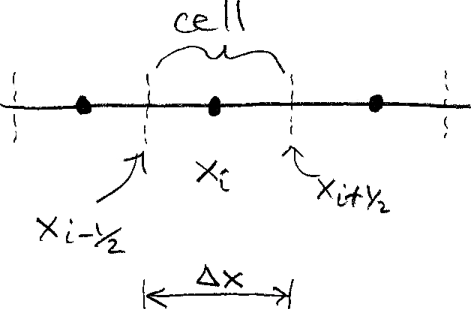
\includegraphics[width=0.35\textwidth]{figs/fvsketch}
\vspace{-4mm}
\item \emph{cell} $=$ \emph{finite volume}
\item suppose $x_i$ is the center of a cell, and integrate over it:
\begin{gather*}
\int_\ximhalf^\xiphalf q_t + f(q)_x \,dx = 0 \hspace{20mm}  \\
\frac{d}{dt} \int_\ximhalf^\xiphalf q(t,x) \,dx + f\left(q(t,\xiphalf)\right) - f\left(q(t,\ximhalf)\right) = 0
\end{gather*}
\end{itemize}
\end{frame}


\begin{frame}{numerical quantities in an FV method}

\begin{itemize}
\item define: \qquad $\ds Q_i(t) \approx \frac{1}{\Delta x} \int_\ximhalf^\xiphalf q(t,x)\,dx$
    \begin{itemize}
    \item[$\circ$] $Q_i(t)$ represents a cell average, not a point value
    \item[$\circ$] versus in a finite difference scheme: $Q_i(t) \approx q(t,x_i)$
    \item[$\circ$] make sure to distinguish $q(t,x_i)$ (exact) and $Q_i(t)$ (numerical)
    \end{itemize}
\item let $\Fiphalf(t) \approx f\left(q(t,\xiphalf)\right)$ be the flux at \emph{cell face}
\item so exact statement from last slide,
$$\frac{d}{dt} \int_\ximhalf^\xiphalf q(t,x) \,dx + f\left(q(t,\xiphalf)\right) - f\left(q(t,\ximhalf)\right) = 0, \hspace{50mm}$$
becomes a numerical scheme:
$$\Delta x \frac{dQ_i}{dt} + \Fiphalf - \Fimhalf = 0 \hspace{50mm}$$
    \begin{itemize}
    \item[$\circ$] this is only a spatial discretization
    \end{itemize}

\vspace{-25mm}
\hfill 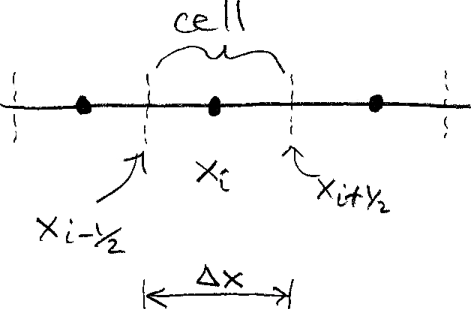
\includegraphics[width=0.3\textwidth]{figs/fvsketch}

\end{itemize}
\end{frame}


\begin{frame}{an almost-complete FV scheme}

\begin{itemize}
\item also put a grid on $t$
\item use forward Euler in time
\item we have this derivation of a scheme:
\small
\begin{gather*}
q_t + f(q)_x = 0 \hspace{50mm} \\
\frac{d}{dt} \int_\ximhalf^\xiphalf q(t,x) \,dx + f\left(q(t,\xiphalf)\right) - f\left(q(t,\ximhalf)\right) = 0 \hspace{50mm} \\
\Delta x \frac{dQ_i}{dt} + \Fiphalf - \Fimhalf = 0 \hspace{50mm} \\
\Delta x \left(\frac{Q_i^{n+1} - Q_i^n}{\Delta t}\right) + \Fiphalfn - \Fimhalfn = 0 \hspace{50mm} \\
\alert{\frac{Q_i^{n+1} - Q_i^n}{\Delta t} + \frac{\Fiphalfn - \Fimhalfn}{\Delta x} = 0} \hspace{50mm}
\end{gather*}

\vspace{-15mm}

\hfill 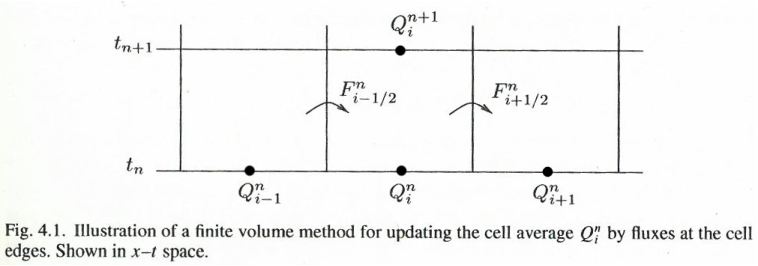
\includegraphics[width=0.45\textwidth]{figs/leveque4p1}

\normalsize
\medskip
\item the \alert{red equation} is a computable numerical scheme \emph{if} we have a scheme for approximating the face fluxes $\Fiphalfn$
\end{itemize}
\end{frame}


\begin{frame}{method-of-lines (MOL) thinking}

\begin{itemize}
\item \emph{but} we should not commit to forward Euler so soon!
\item remember: $\ds Q_i(t) \approx \frac{1}{\Delta x} \int_\ximhalf^\xiphalf q(t,x)\,dx$ and $\Fiphalf(t) \approx f\left(q(t,\xiphalf)\right)$
\item  our basic FV scheme is an ODE system in time:
    $$\frac{dQ_i}{dt} + \frac{\Fiphalf-\Fiphalf}{\Delta x} = 0 \hspace{60mm}$$

\vspace{-15mm}
\hfill 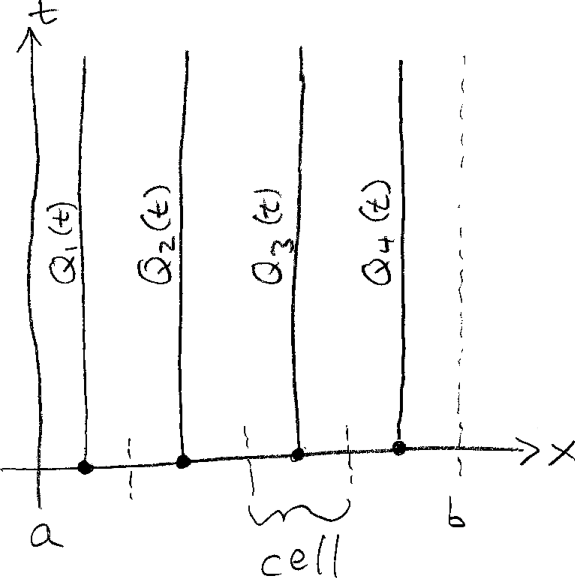
\includegraphics[width=0.3\textwidth]{figs/molsketch}

\vspace{-21mm}
\item write as:
    $$\frac{d\bQ}{dt} = \bG(t,\bQ), \quad \bQ(t) = \begin{bmatrix} Q_1(t) \\ \vdots \\ Q_J(t) \end{bmatrix}   \hspace{60mm}$$

\item why? because good black-box ODE solvers are available
    \begin{itemize}
    \item[$\circ$] \dots it is not 1970 anymore, people!
    \end{itemize}
\end{itemize}
\end{frame}


\begin{frame}{upwind as the ``donor cell'' method}

\begin{itemize}
\item in FV language, upwind for $q_t + a q_x = 0$ is 3 steps:
    \begin{itemize}
    \item[i)] integrate over the spatial cell ($=$ derive the FV MOL scheme):
        $$\frac{dQ_i}{dt} + \frac{\Fiphalf-\Fimhalf}{\Delta x} = 0 \hspace{50mm}$$
    \item[ii)] compute flux $F(q)=aq$ from the upwind \emph{donor cell}:
        $$\Fiphalf = \begin{cases} a Q_{i}, & a \ge 0, \\
                                   a Q_{i+1}, & a < 0 \end{cases} \hspace{50mm}$$
    \item[iii)] forward Euler for time stepping:
        $$\frac{Q_i^{n+1} - Q_i^n}{\Delta t} + a \frac{\begin{Bmatrix} Q^n_{i}-Q^n_{i-1} \quad [a\ge 0] \\ Q^n_{i+1}-Q^n_{i} \quad [a<0] \end{Bmatrix}}{\Delta x} = 0 \hspace{50mm}$$
    \end{itemize}

\vspace{-30mm}

\hfill 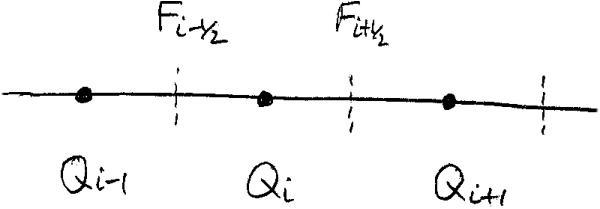
\includegraphics[width=0.4\textwidth]{figs/cellfluxsketch}

\vspace{12mm}
\item for ii) we will do better {\small (``high-resolution'' methods; ``slope-limiters'')}
    \begin{itemize}
    \item[$\circ$] but how to interpret ``donor cell'' for hyperbolic \emph{systems}?
    \end{itemize}
\item for iii) we can already do better {\small (Runge-Kutta, Matlab ODE solvers, \dots)}
\end{itemize}
\end{frame}


\section{linear systems and Riemann solvers}

\begin{frame}{linear systems: examples}

\begin{itemize}
\item consider a \emph{linear, constant-coefficient, homogeneous system}:
  $$\bq_t + A\, \bq_x=0$$

    \begin{itemize}
    \item[$\circ$] $\bq(t,x) \in \RR^d$ vector-valued solution
    \item[$\circ$] $A\in\RR^{d\times d}$ square matrix
    \end{itemize}
 
\bigskip
\setlength{\itemindent}{21mm}
\item[$d=2$ example:] \emph{acoustics} ($=$ classical 2nd-order wave equation)
        $$\bq = \begin{bmatrix} p \\ u \end{bmatrix}, \,\, A = \begin{bmatrix} 0 & K_0 \\ \frac{1}{\rho_0} & 0 \end{bmatrix} \quad \implies \quad \begin{matrix} p_t + K_0 u_x = 0 \\ u_t + \frac{1}{\rho_0} p_x = 0 \end{matrix}$$
\item[$d=2$ example:] \underline{linearized} \emph{shallow water equations}
        $$\bq = \begin{bmatrix} h \\ h u \end{bmatrix}, \,\, A = \begin{bmatrix} 0 & 1 \\ -u_0^2+gh_0 & 2 u_0 \end{bmatrix} \, \implies \, {\footnotesize \begin{matrix} {\large \strut} h_t + (hu)_x = 0 \\ {\large \strut} (h u)_t + (-u_0^2+gh_0) h_x + 2u_0 (h u)_x = 0 \end{matrix} }$$
\end{itemize}
\end{frame}


\begin{frame}{example: acoustics}

\begin{itemize}
\item $p(t,x)$ is gas pressure, $u(t,x)$ is gas velocity
\item assume pressure/velocity variations are small, and density $\rho_0$ and compressiblity $K_0$ are constant
\item thus linear, constant-coefficient first-order PDE system:
$$\begin{matrix} p_t + K_0 u_x = 0 \\ u_t + \frac{1}{\rho_0} p_x = 0 \end{matrix} \hspace{70mm}$$
\item or $\bq_t + A \bq_x=0$ where
$$\bq = \begin{bmatrix} p \\ u \end{bmatrix}, \, A = \begin{bmatrix} 0 & K_0 \\ \frac{1}{\rho_0} & 0 \end{bmatrix} \hspace{75mm}$$
\item or in 2nd-order form

with $c^2 = \frac{K_0}{\rho_0}$:
\begin{align*}
p_{tt} &= c^2 p_{xx} \hspace{70mm} \\
u_{tt} &= c^2 u_{xx}
\end{align*}
\item example solution $\longrightarrow$

\vspace{-60mm}
\hfill 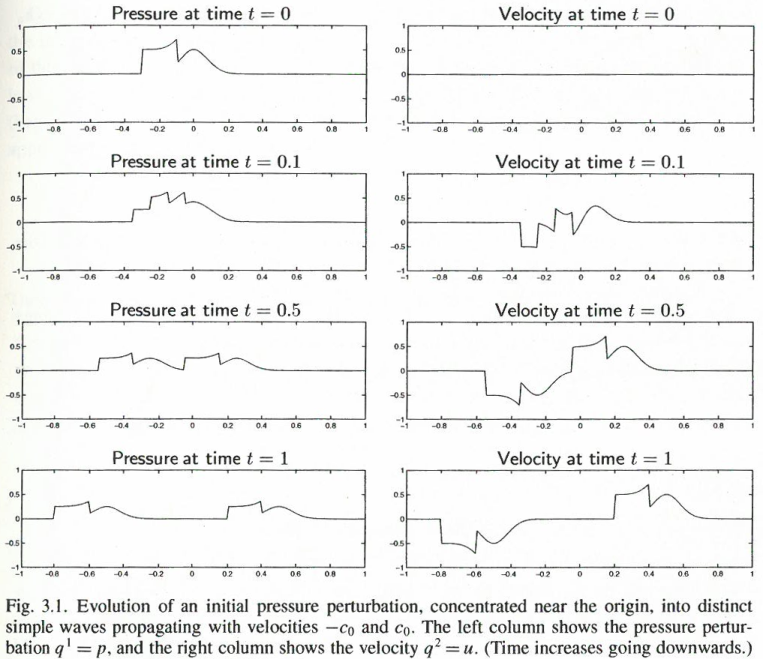
\includegraphics[width=0.55\textwidth]{figs/leveque3p1}
\end{itemize}
\end{frame}


\begin{frame}{linear system we can already handle}

\begin{itemize}
\item consider boring decoupled system:
        $$\bq = \begin{bmatrix} u \\ v \\ w \end{bmatrix}, \,\, A = \begin{bmatrix} a & 0 & 0 \\ 0 & b & 0 \\ 0 & 0 & c \end{bmatrix} \, \implies \begin{matrix} u_t + a u_x = 0 \\ v_t + b v_x = 0 \\ w_t + c w_x = 0 \end{matrix}$$
\item \emph{method}: upwind on each equation independently

\bigskip
\item \emph{claim}: for general $A$, changing the basis should put us in this boring situation
\item notation: bold for column vectors $\bu\in\RR^d$
    \begin{itemize}
    \item[$\circ$] inner product: \quad $\bu^\top \bv = \ip{\bu}{\bv}$
    \end{itemize}
\end{itemize}
\end{frame}


\begin{frame}{hyperbolic systems}

\begin{definition} a first-order system $\bq_t + A\, \bq_x=0$ is \emph{hyperbolic} if $A$ is diagonalizable and all of the eigenvalues of $A$ are real
\end{definition}

\begin{itemize}
\item \emph{diagonalizable} $=$ there is a basis of $\RR^d$ consisting of eigenvectors of $A$
\item consider \emph{left eigenvectors} of $A$, namely vectors $\bw_k \in \RR^d$ so that
    $$\bw_k^\top A = \lambda_k \bw_k^\top$$

\vspace{-2mm}
    \begin{itemize}
    \item[$\circ$] $\lambda_k$ are \emph{eigenvalues}, real numbers if the system is hyperbolic
    \item[$\circ$] $\bw_k$ are column vectors so $\bw_k^\top$ are row vectors
    \item[$\circ$] $\bw_k$ are also right eigenvectors of $A^\top$: \qquad $A^\top \bw_k = \lambda_k \bw_k$
    \item[$\circ$] the left/right eigen\emph{values} are the same
    \end{itemize}
\end{itemize}
\end{frame}


\begin{frame}{eigenvectors decouple hyperbolic systems}

\begin{itemize}
\item assume the system $\bq_t + A\, \bq_x=0$ is hyperbolic
\item decouple it by multiplying by $\bw_k^\top$:
\begin{align*}
\bw_k^\top \bq_t + \bw_k^\top A\, \bq_x &= 0 \\
\bw_k^\top \bq_t + \lambda_k \bw_k^\top \bq_x &= 0
\end{align*}
\item define scalar functions (inner products)
    $$v_k(t,x) = \bw_k^\top \bq(t,x)$$
\item these scalar functions satisfy decoupled advection equations:
   $$(v_k)_t + \lambda_k (v_k)_x = 0$$
\item solve these one-way advection problems by characteristics:
   $$v_k(t,x) = v_k(0,x-\lambda_k t)$$
\item \emph{note}: \alert{matrix $A$ must be constant for this calculation}
\end{itemize}
\end{frame}


\begin{frame}{eigenvectors decouple hyperbolic systems $=$ Riemann invariants}

\begin{itemize}
\item the functions $v_k(t,x)$ are called the \emph{Riemann invariants}:
    $$v_k(t,x) = \bw_k^\top \bq(t,x) = v_k(0,x-\lambda_k t) = \bw_k^\top \bq(0,x-\lambda_k t)$$

\item but how to write $\bq(t,x)$ if we have $v_k(t,x)$?
    \begin{itemize}
    \item[$\circ$] expand in basis $\bw_k$, with scalar coefficients $c_k(t,x)$:
    $$\alert{\bq(t,x) = \sum_{k=1}^d c_k(t,x) \bw_k}$$
    \item[$\circ$] note \qquad $\ds v_\ell(t,x) = \bw_\ell^\top \bq(t,x) = \sum_{k=1}^d c_k(t,x) \bw_\ell^\top \bw_k$
    \item[$\circ$] define matrix $B\in \RR^{d\times d}$ with entries \alert{$B_{\ell k} = \bw_\ell^\top \bw_k$}:
    \item[$\circ$] $B$ is invertible so solve:
    $$B \bc = \bv \qquad \iff \qquad \alert{\sum_{k=1}^d B_{\ell k} c_k(t,x) = \bw_\ell^\top \bq(0,x-\lambda_\ell t)}$$
    \end{itemize}
\item \alert{red equations} combine into a computable solution
\end{itemize}
\end{frame}


\begin{frame}[fragile]
\frametitle{left eigenvectors, transposes, and \Matlab}

\begin{itemize}
\item left eigenvectors for $A$ are the same as right eigenvectors for $A^\top$
\item in \Matlab, find left eigenvectors $\bw_k$ by applying \texttt{eig()} to \texttt{A'}$=A^\top$:
\begin{Verbatim}[fontsize=\small]
>> A = [...; ...; ...];     % input square matrix A
>> [X,D] = eig(A');
>> lamk = D(k,k);           % eigenvalue
>> wk = X(:,k);             % left eigenvector
\end{Verbatim}
\end{itemize}
\end{frame}


\begin{frame}{Riemann solver}

\begin{itemize}
\item key idea: in a FV scheme, at $t_n$ we have \alert{two different numerical values on either side of the cell face} at $x_{i+1/2}$:
    $$\bQ_{i} = \bQ_L, \quad \bQ_{i+1} = \bQ_R \hspace{50mm}$$

\vspace{-12mm}
\hfill 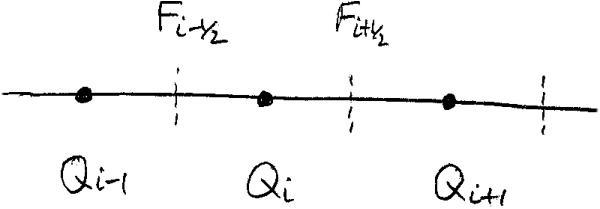
\includegraphics[width=0.4\textwidth]{figs/cellfluxsketch}

\medskip
\item on the other hand: $\bbf(\bq) = A\bq$ is a function of $\bq$, so to get flux $\bF_{i+1/2}$ we must know the solution \emph{on} the face: $\bq(t,x_{i+1/2})$ for $t > t_n$
\item a \emph{Riemann solver} solves the following problem:

\bigskip
find $\bq(t,x_{i+1/2})$ for $t > t_n$ given
\begin{align*}
\bq_t + \bbf(\bq)_x &= 0 \\
\bq(t_n,x) &= \begin{cases} \bQ_L, & x < x_{i+1/2} \\
                            \bQ_R, & x > x_{i+1/2} \end{cases} \hspace{60mm}
\end{align*}

\vspace{-30mm}
\hfill 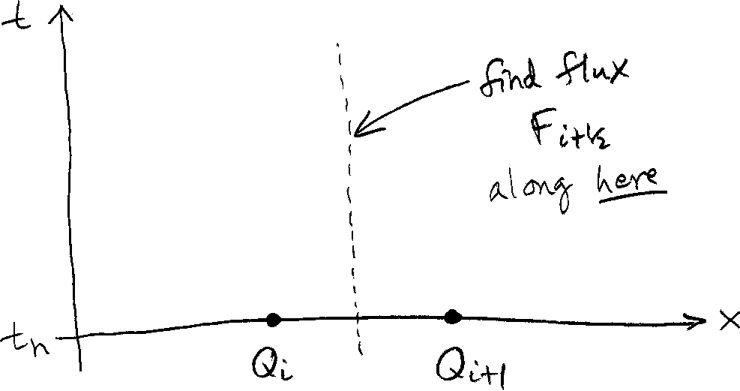
\includegraphics[width=0.44\textwidth]{figs/rsolversketch}
\end{itemize}
\end{frame}


\begin{frame}{forward versus backward characteristics}

\begin{itemize}
\item thus when constructing numerical schemes for hyperbolic problems there are two ways of thinking about characteristics:
    \begin{itemize}
    \item[i)] Riemann solvers generate a flux at $x_*$ at times $t>t_n$
    \item[ii)] FD methods (e.g.~Lax-Wendroff) find $(x_j,t_{n+1})$ solution by going back to $t_n$
    \end{itemize}
\item 

\medskip

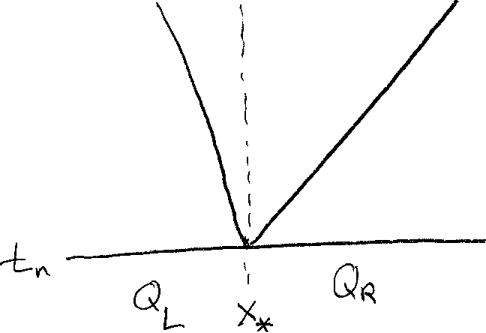
\includegraphics[height=0.34\textheight]{figs/rscharssketch} \hfill 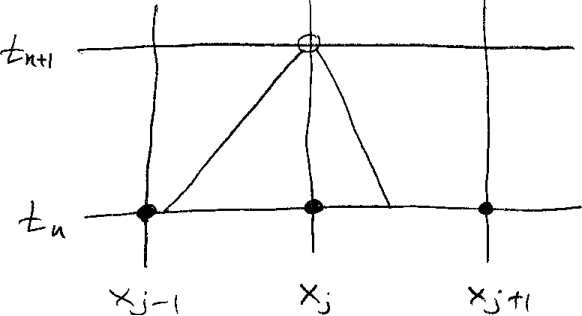
\includegraphics[height=0.38\textheight]{figs/fdcharssketch}

\medskip
\qquad Riemann solver view \hfill finite difference (FD) view \qquad \phantom{x}

\item the Riemann solver view makes it easier to
    \begin{itemize}
    \item[$\circ$] generalize to nonlinear systems
    \item[$\circ$] work with the MOL equations (because no time-step choice)
    \end{itemize}
\end{itemize}
\end{frame}


\begin{frame}{Riemann solver for the acoustics problem}

\begin{itemize}
\item for example, \dots
\item recall the acoustics problem $\bq_t + A \bq_x = 0$:
        $$\bq = \begin{bmatrix} p \\ u \end{bmatrix}, \,\, A = \begin{bmatrix} 0 & K_0 \\ \frac{1}{\rho_0} & 0 \end{bmatrix} \quad \implies \quad \begin{matrix} p_t + K_0 u_x = 0 \\ u_t + \frac{1}{\rho_0} p_x = 0 \end{matrix}$$
\item eigen-decomposition of $A$:
\begin{align*}
\lambda_1 &= -c_0, \quad \bw_1 = \begin{bmatrix} 1 \\ -Z_0 \end{bmatrix} & \lambda_2 = +c_0, \quad \bw_2 = \begin{bmatrix} 1 \\ +Z_0 \end{bmatrix}
\end{align*}
where \, $c_0 = \sqrt{K_0/\rho_0}$ \, and \, $Z_0=\rho_0 c_0$
\item thus the Riemann invariants $v_k(t,x) = \bw_k^\top \bq(t,x)$ are:
\begin{align*}
v_1(t,x) &= p(t,x) - Z_0 u(t,x), & v_2(t,x) &= p(t,x) + Z_0 u(t,x)
\end{align*}
\end{itemize}
\end{frame}


\begin{frame}{Riemann solver for the acoustics problem 2}

\begin{itemize}
\item denote $x_*=x_{i+1/2}$ and let $\quad \bQ_L = \begin{bmatrix} p_L \\ u_L \end{bmatrix}, \quad \bQ_R = \begin{bmatrix} p_R \\ u_R \end{bmatrix}$
\item $\lambda_1 < 0$ so $v_1$ is left-going, so we solve forward from $t=t_n$:
\begin{align*}
p(t,x_*) - Z_0 u(t,x_*) &= v_1(t,x_*) = v_1(t_n,x_*-\lambda_1 (t-t_n)) \\
   &= p_R - Z_0 u_R
\end{align*}
\item $\lambda_2 > 0$ so $v_2$ is right-going:
\begin{align*}
p(t,x_*) + Z_0 u(t,x_*) &= v_2(t,x_*) = v_2(t_n,x_*-\lambda_2 (t-t_n)) \\
   &= p_L - Z_0 u_L
\end{align*}
\item solve for the solution at the face, namely $\bq(t,x_*)$:
\begin{align*}
\alert{p(t,x_*)} &\alert{= \frac{1}{2} \left(p_L + p_R + Z_0 (u_L - u_R)\right)} \\
\alert{u(t,x_*)} &\alert{= \frac{1}{2} \left(\frac{1}{Z_0} (p_L - p_R) + u_L + u_R)\right)}
\end{align*}
\item thus the face flux at $x_*=x_{i+1/2}$ is computable; this is the Riemann solver:
    $$\alert{\bF_{i+1/2}(t) =} A \bQ(t,x_*) = \alert{\begin{bmatrix} K_0 u(t,x_{i+1/2}) \\ \frac{1}{\rho_0} p(t,x_{i+1/2}) \end{bmatrix}}$$
\end{itemize}
\end{frame}


\begin{frame}{flux boundary conditions, and the grid}

\begin{itemize}
\item boundary conditions at $x=a,b$
\item easiest if think in terms of the value of the \emph{flux} there,
\item \dots thus we set up the grid to have cell faces at $x=a,b$

\medskip
\begin{center}
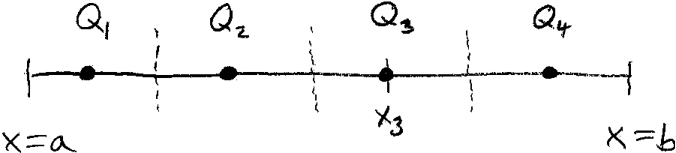
\includegraphics[width=0.45\textwidth]{figs/fluxbdrysketch}
\end{center}

\vspace{-2mm}
    $$x_j = a + (j-1/2) \Delta x \quad \text{ where } \quad \Delta x = \frac{b-a}{J}$$

\item for the acoustics problem on the next slide, suppose
    \begin{itemize}
    \item[$\circ$] reflecting condition on left: $u(t,a)=0$
    \item[$\circ$] outflow condition on right: $v_1(t,b)=0$
    \end{itemize}
\item modify the Riemann solvers at $x=a$ and $x=b$ accordingly
    \begin{itemize}
    \item[$\circ$] inflow versus outflow condition is clear in the scheme
    \end{itemize}
\end{itemize}
\end{frame}


\begin{frame}{demonstration of acoustics solver}

\begin{itemize}
\item I used all these ideas in a C$+$PETSc program for the acoustics problem
\item see \texttt{riemann} at
\begin{center}
\href{https://github.com/bueler/p4pdes-next}{\texttt{github.com/bueler/p4pdes-next}}
\end{center}

\vspace{3mm}
\begin{center}
\alert{SHOW ACOUSTICS MOVIE}
\end{center}
\end{itemize}

% ./riemann -da_grid_x 500 -ts_max_time 5 -limiter mc -ts_monitor binary:t.dat -ts_monitor_solution binary:q.dat
% make petscPyScripts
% mkdir acoustic
% ./plotTS.py -mx 500 -dof 2 -c 0 -ylabel "p (pressure)" -ax -1.0 -bx 1.0 -cellcentered -oroot acoustic/bar t.dat q.dat
% cd acoustic/
% eog bar*.png
\end{frame}


\begin{frame}{summary of linear hyperbolic systems and Riemann solvers}

\begin{itemize}
\item if a linear system $\bq_t + A\, \bq_x=0$ in $\RR^d$ is \alert{\emph{hyperbolic}} then (by definition) it can be decoupled ($\bw_k^\top A = \lambda_k \bw_k$) into $d$ scalar (real) advection problems
\item the solutions of these advection problems, forward from time $t_n$, are the \alert{\emph{Riemann invariants}}:
    $$v_k(t,x) = \bw_k^\top \bq(t,x) = v_k(t_n,x-\lambda_k (t-t_n))$$
\item now write in conservation form: $\bq_t + \bbf(\bq)_x=0$ where $\bbf(\bq) = A\bq$
\item in the FV \alert{\emph{method-of-lines (MOL)}} view we only integrate in space:
    $$\frac{d\bQ_j}{dt} + \frac{\bF_{i+1/2} - \bF_{i-1/2}}{\Delta x} = 0$$
\item a \alert{\emph{Riemann solver}} finds the face fluxes $\bF_{i+1/2}=A \bQ^*$ by solving the \emph{Riemann problem}, with $\bQ_L,\bQ_R$ on sides of the face, to find $\bQ^*$ on the face
    \begin{itemize}
    \item[$\circ$] this uses the Riemann invariants
    \end{itemize}

\bigskip
\footnotesize
\item generalize to nonlinear systems by using $A=\bbf'(\bq)$?
\end{itemize}
\end{frame}


\section{high-resolution methods (slope-limiters)}

\begin{frame}{Godunov's barrier theorem}

\begin{itemize}
\item can we do better than Lax-Wendroff, even for scalar advection?
\item can we have high accuracy without oscillations?
    \begin{itemize}
    \item[$\circ$] upwinding is only first-order accurate, but it avoids oscillations
    \item[$\circ$] Lax-Wendroff is second-order but it generates oscillations beyond the range of the initial condition
    \end{itemize}
\item rough answer: \only<1>{\alert{NO}}\only<2>{\cancel{NO} \alert{yes}}

\medskip
\begin{theorem}[\emph{Godunov, 1959}]  A monotonicity-preserving \alert<2>{linear} scheme for $q_t + a q_x=0$ cannot have second-order (or higher) local truncation error in $x$.\end{theorem}

\item ``monotonicity-preserving'' means (essentially) that the scheme does not add oscillations
\item Godunov's barrier created modern hyperbolic PDE solvers
    \begin{itemize}
    \item[$\circ$] upwinding, Lax-Friedrichs, Lax-Wendroff, leapfrog are the old technology
    \item[$\circ$] ``high-resolution'' schemes of the 1970--90s overcame the barrier \only<2>{\quad \alert{how?}}
    \end{itemize}
\end{itemize}
\end{frame}


\begin{frame}{the reconstruct-evolve-average view of FV schemes}

\begin{itemize}
\item if we want to kill oscillation then another view is helpful
\item consider: $q_t + a q_x=0$ for $a>0$, with cell values $\{Q_i^n\}$
\item apply 1st-order upwinding Euler step from $t_n$ (left) to $t_{n+1}$ (right):

\begin{center}
\quad 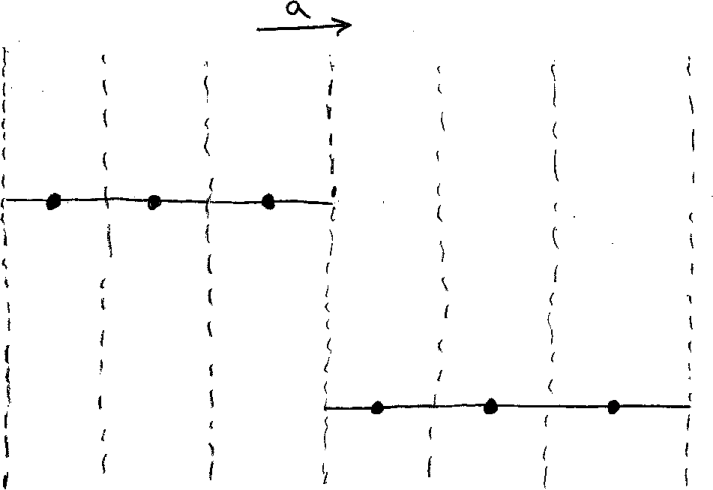
\includegraphics[width=0.3\textwidth]{figs/upreconstructleft} \qquad 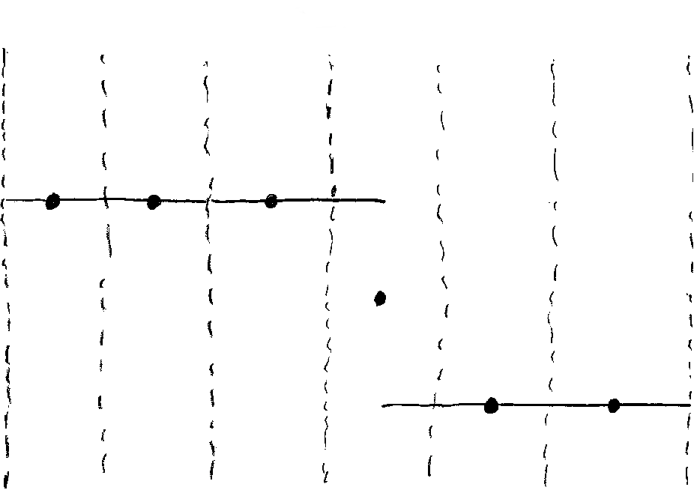
\includegraphics[width=0.3\textwidth]{figs/upreconstructright}
\end{center}

    \begin{itemize}
    \item[$\circ$] right figure: new cell averages (dots) after evolving exact solution (lines)
    \item[$\circ$] upwinding uses constant values in cells (\emph{see next slide})
    \end{itemize}
\item versus Lax-Wendroff, which uses downwind slope:

\begin{center}
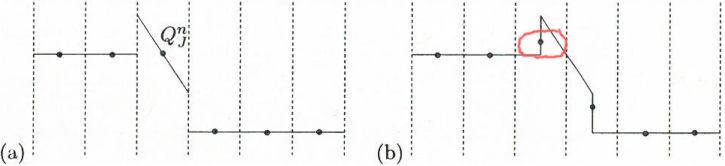
\includegraphics[width=0.69\textwidth]{figs/leveque6p4}
\end{center}

    \begin{itemize}
    \item[$\circ$] note the \alert{overshoot}, which we want to avoid
    \end{itemize}
\end{itemize}
\end{frame}


\begin{frame}{slope reconstruction}

\begin{itemize}
\item at time $t_n$ we only have the discrete unknowns $\{Q_j^n\}$
\item but we can ``reconstruct'' a linear function $\tilde q(t_n,x)$ on each cell:
    $$\tilde q(t_n,x) = Q_i^n + \sigma_i^n (x - x_i)$$

    \begin{itemize}
    \item[$\circ$] $\sigma_i^n$ is the \emph{slope} in the cell $[x_{i-\frac{1}{2}}, x_{i+\frac{1}{2}}]$
    \item[$\circ$] for any $\sigma_i^n$, the cell average remains $Q_i^n$
    \end{itemize}

\medskip
\item possibilities for slope when $a>0$:
\begin{align*}
&\text{zero:}     & \sigma_i &= 0 \hspace{75mm} \\
&\text{{\color{red} downwind:}} & \sigma_i &= \frac{Q_{i+1}-Q_i}{\Delta x} \\
&\text{{\color{ForestGreen} upwind:}}   & \sigma_i &= \frac{Q_i-Q_{i-1}}{\Delta x} \\
&\text{{\color{blue} centered:}} & \sigma_i &= \frac{Q_{i+1}-Q_{i-1}}{2\Delta x}
\end{align*}

\vspace{-45mm}
\hfill 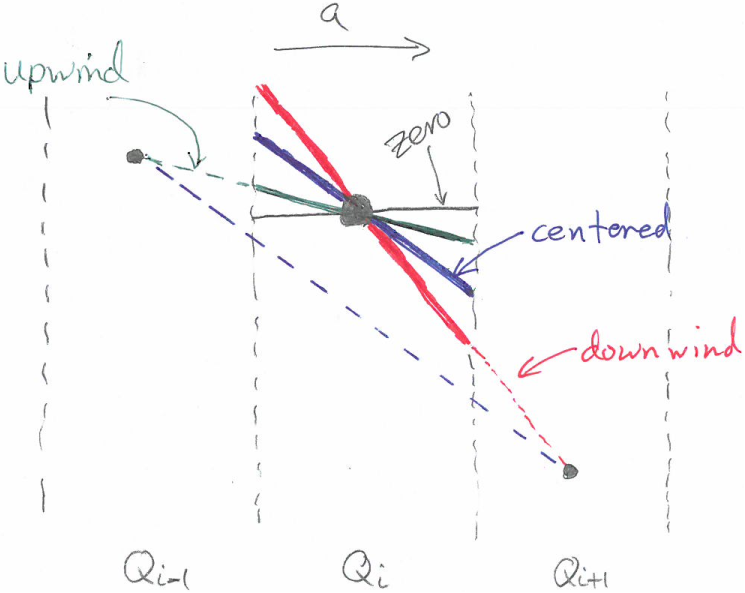
\includegraphics[width=0.47\textwidth]{figs/slopessketch}

\footnotesize
\item \alert{WARNING:} upwind \emph{scheme} uses zero slope
\end{itemize}
\end{frame}


\begin{frame}{from reconstruction to flux}

\begin{itemize}
\item for slope $\sigma_i^n$ we get a model (reconstruction) of the solution in the cell:
    $$\tilde q(t_n,x) = Q_i^n + \sigma_i^n (x - x_i)$$
\item this gives solution estimates at the cell faces $x_{i-1/2},x_{i+1/2}$:
    $$Q^L_i = \tilde q(t_n,x_{i-1/2}) = Q_i^n - \sigma_i^n \frac{\Delta x}{2}$$
    $$Q^R_i = \tilde q(t_n,x_{i+1/2}) = Q_i^n + \sigma_i^n \frac{\Delta x}{2}$$
    \begin{itemize}
    \item[$\circ$] use these to compute the fluxes at cell faces in an explicit method
    \end{itemize}
\item for example, in the scalar advection equation $F(q)=aq$:
    $$F_{i+\half}=\begin{cases} a Q^R_i, & a \ge 0 \\
                                a Q^L_{i+1}, & a < 0\end{cases}$$
    \begin{itemize}
    \item[$\circ$] similarly for $F_{i-\half}$
    \item[$\circ$] compare the ``upwind as the donor cell method'' slide
    \end{itemize}
\end{itemize}
\end{frame}


\begin{frame}{slope limiter idea}

\begin{itemize}
\item we should use a nonzero slope $\sigma_i$ to get higher accuracy
\item \dots \emph{except} when the slope would put the reconstruction out of range of the three values $\{Q_{i-1},Q_i,Q_{i+1}\}$
\item computing $\sigma_i$ by a \emph{slope limiter} avoid the out-of-range problem
\item for example, the \alert{$\minmod$ \emph{slope limiter}:}
    $$\sigma_i = \minmod\left\{\frac{Q_i-Q_{i-1}}{\Delta x},\frac{Q_{i+1}-Q_i}{\Delta x}\right\}$$

    \begin{itemize}
    \item[$\circ$] by definition, for real numbers $a,b$ of the same sign:
        $$\minmod\{a,b\} = \begin{cases} 0, & ab \le 0 \\
                                         a, & ab>0 \text{ and } |a| \le |b| \\
                                         b, & ab>0 \text{ and } |a| > |b| \end{cases}$$
    \item[$\circ$] in words: $\minmod\{a,b\}$ is closest to zero of $a$ and $b$ unless they differ in sign; then it is zero
    \item[$\circ$] if $Q_i$ is the extrema of the three values then $\sigma_i = 0$
    \end{itemize}
\end{itemize}
\end{frame}


\begin{frame}{slope limiter idea 2}

\begin{itemize}
\item an alternative is the \alert{\emph{MC slope limiter}:}
    $$\sigma_i = \minmod\left\{\frac{Q_{i+1}-Q_{i-1}}{2\Delta x},2\minmod\Big\{\frac{Q_i-Q_{i-1}}{\Delta x},\frac{Q_{i+1}-Q_i}{\Delta x}\Big\}\right\}$$
\item in pictures:

\begin{center}
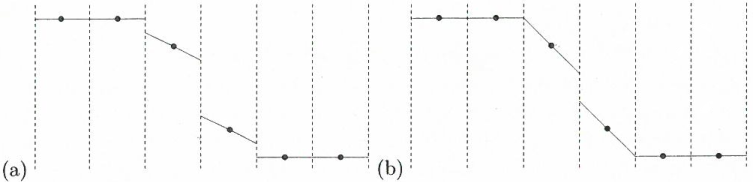
\includegraphics[width=0.9\textwidth]{figs/leveque6p5}
\end{center}

\hspace{15mm} $\minmod$ limiter \hfill MC limiter \hspace{15mm} \phantom{x}

\medskip
    \begin{itemize}
    \item[$\circ$] can you draw-in the downwind slopes (Lax-Wendroff)?  \dots get overshoot
    \end{itemize}

\medskip
\footnotesize
\item historical comment: the theory of \emph{total variation diminishing} (TVD) schemes, circa 1990s, arises from these pictures
\end{itemize}
\end{frame}


\begin{frame}{results for advection equation}

\begin{itemize}
\item consider scalar advection again: $q_t + a q_x=0$, $a=1$, periodic b.c.s
\end{itemize}

\begin{center}
\includegraphics<1>[width=0.7\textwidth]{figs/leveque6p1} \includegraphics<2>[width=0.7\textwidth]{figs/leveque6p2}
\end{center}
\end{frame}


\begin{frame}{MOL: slope limiting and Riemann solvers}

\begin{itemize}
\item suppose we want to use limited slopes and Riemann solvers in a method-of-lines (MOL) framework \dots how to do this?
\item \emph{answer}: apply the slope calculation and slope-limiter as usual and then compute the flux $F_{i-1/2}$ in terms of this picture:

\medskip
\begin{center}
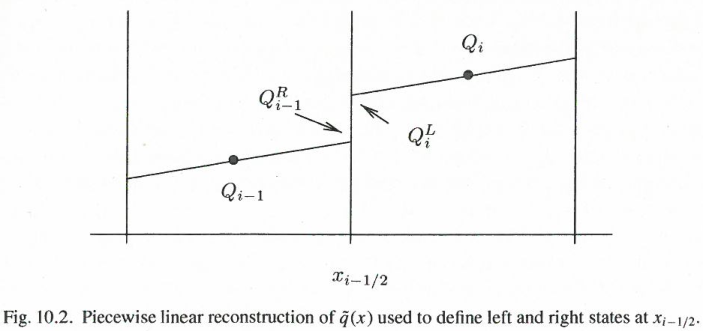
\includegraphics[width=0.6\textwidth]{figs/leveque10p2}
\end{center}
\item the left and right values at the face, $Q_{i-1}^R$ and $Q_i^L$, are the ones used in the Riemann solver to compute the solution value at the face for $t>t_n$
\item thereby get the flux $F_{i-1/2}(t)$ for $t>t_n$
\end{itemize}
\end{frame}


\section{nonlinear conservation laws}

\begin{frame}{conservation laws}

\begin{itemize}
\item a \emph{conservation law} is a first-order PDE system, for $\bq(t,x) \in \RR^d$, with a given \emph{flux function} $\bbf$ and \emph{source function} $\bg$:
  $$\bq_t + \bbf(t,x,\bq)_x=\bg(t,x,\bq)$$
    \begin{itemize}
    \item[$\circ$] linear conservation law: \qquad $\bbf(\bq) = A\bq$
    \item[$\circ$] if $\bbf$ depends on $\grad \bq$ (e.g.~heat equation) then the system is \emph{not} hyperbolic
    \end{itemize}

\bigskip
\item scalar, nonlinear, and hyperbolic examples:
    \begin{itemize}
    \item[$\circ$] \emph{Burger's equation} with $f(q)=\frac{1}{2} q^2$ and $g=0$:
        $$q_t + \left(\tfrac{1}{2} q^2\right)_x = 0 \qquad \iff \qquad q_t + q q_x = 0$$
    \item[$\circ$] \emph{nonlinear traffic model} with $f(q)=u_{\max} (1-q) q$ and $g=0$:
        $$q_t + \left(u_{\max} (1-q) q\right)_x = 0$$
    \end{itemize}
\end{itemize}
\end{frame}


\begin{frame}{nonlinear conservation laws: system examples}

\begin{itemize}
\item \emph{shallow water equations} with height $h(t,x)$ and velocity $u(t,x)$:
        $$\bq = \begin{bmatrix} h \\ hu \end{bmatrix}, \, \bbf(\bq) = \begin{bmatrix} hu \\ h u^2 + \frac{g}{2} h^2 \end{bmatrix} \quad \implies \quad \begin{matrix} h_t + (hu)_x = 0 \\ (hu)_t + \Big(h u^2 + \frac{g}{2} h^2\Big)_x = 0 \end{matrix}$$
\item \emph{Euler equations for an ideal gas}:
        $$\bq = \begin{bmatrix} \rho \\ \rho u \\ E \end{bmatrix}, \, \bbf(\bq) = \begin{bmatrix} \rho u \\ \rho u^2 + p \\ (E+p) u \end{bmatrix} \quad \implies \quad \begin{matrix} \rho_t + (\rho u)_x = 0 \\ (\rho u)_t + \Big(\rho u^2 + p\Big)_x = 0 \\ E_t + \Big((E+p) u\Big)_x = 0 \end{matrix}$$
    \begin{itemize}
    \item[$\circ$] variables are density $\rho(t,x)$, velocity $u(t,x)$, and energy density $E(t,x)$
    \item[$\circ$] the pressure $p$ is found from an equation of state, for example for a polytropic ideal gas ($\gamma \approx 1.4$ for air):
        $$E = \frac{p}{\gamma - 1} + \frac{1}{2} \rho u^2$$
    \end{itemize}
\end{itemize}
\end{frame}


\begin{frame}{scalar conservation law: traffic model}

\begin{itemize}
\item for this traffic model, $q(t,x)$ is the density of cars, $0\le q \le 1$
\item cars move at speed
    $$U(q) = u_{\max} (1-q)$$

    \begin{itemize}
    \item[$\circ$] they slow down when the density is high
    \end{itemize}
\item the flux of cars is
    $$f(q) = U(q) q = u_{\max} (1-q) q$$
\item but note that
    $$f'(q) = u_{\max} (1-2q)$$
\item scalar nonlinear conservation laws are nonlinear advection problems:
    $$q_t + f'(q) q_x = 0$$
\item the solution is constant along characteristics, but the characteristic speed depends on the solution:
    $$a = f'(q) = u_{\max} (1-2q)$$
\end{itemize}
\end{frame}


\begin{frame}{traffic: speed versus speed}

\begin{itemize}
\item speed of car is $U(q) = u_{\max} (1-q)$
\item speed of characteristic is $f'(q) = u_{\max} (1-2q)$
\end{itemize}

\begin{center}
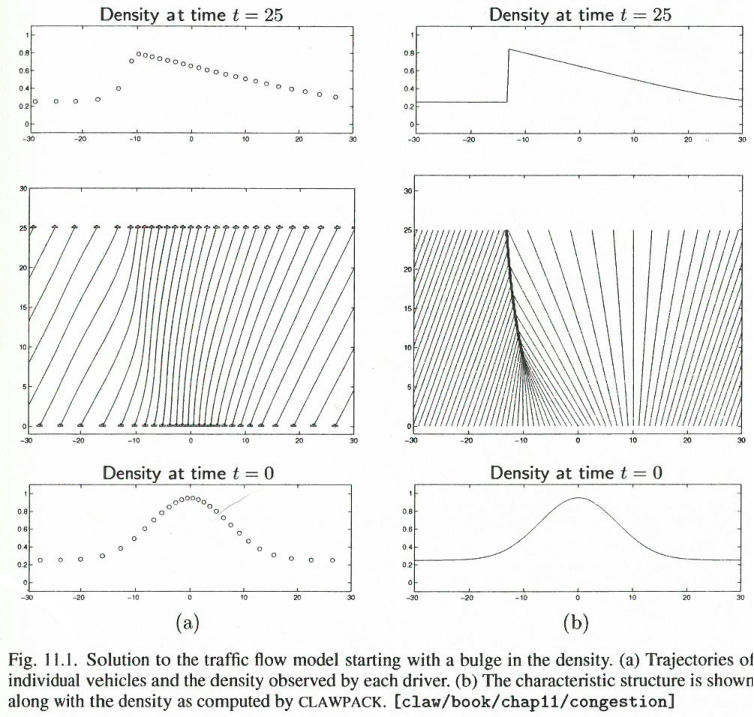
\includegraphics[width=0.68\textwidth]{figs/leveque11p1}
\end{center}
\end{frame}


\begin{frame}{traffic: shock and rarefaction waves}

\begin{itemize}
\item previous slide shows formation of a \emph{shock wave} from a smooth hump
\item the model can also form \emph{rarefaction waves}
\end{itemize}

\begin{center}
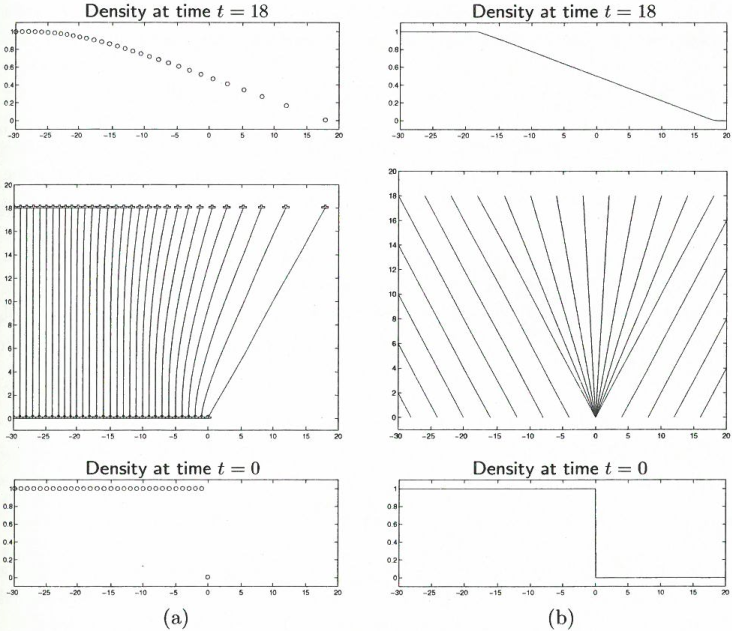
\includegraphics[width=0.65\textwidth]{figs/leveque11p3}
\end{center}
\end{frame}


\begin{frame}{recall the FV-MOL-Riemann solver idea}

\begin{itemize}
\item for problems in flux-conservation form: \quad $q_t + f(q)_x = 0$
\item put a grid on $x$, with $x_i$ at cell center
\item integrate over the cell:
    $$\frac{d}{dt} \int_\ximhalf^\xiphalf q(t,x) \,dx + f\left(q(t,\xiphalf)\right) - f\left(q(t,\ximhalf)\right) = 0$$
\item interpret discrete unknowns as cell averages (FV):
    $$Q_i(t) = \frac{1}{\Delta x} \int_\ximhalf^\xiphalf q(t,x)\,dx$$
\item get a big ODE system (MOL) for solution by an ODE black box:
    $$\frac{dQ_i}{dt} + \frac{F_{i+1/2} - F_{i-1/2}}{\Delta x} = 0$$
\item a (slope-limited) Riemann solver will compute the face fluxes $F_{i+1/2}$
\end{itemize}
\end{frame}


\begin{frame}{Riemann problem for scalar conservation laws}

\begin{itemize}
\item the Riemann problem addresses a discontinuity at $x_*=x_{i+1/2}$:
    $$q_t + f'(q)q_x = 0, \qquad q(t_n,x) = \begin{cases} Q_L & x < x_* \\ Q_R & x > x_* \end{cases}$$

    \begin{itemize}
    \item[$\circ$] the goal is to compute $Q_*$ on the face at $x_*$
    \item[$\circ$] and thereby compute the flux $F_{i+1/2}$
    \end{itemize}
\item for scalar nonlinear conservation laws there are several possibilities:

\begin{center}
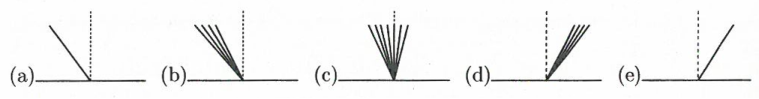
\includegraphics[width=0.75\textwidth]{figs/leveque12p1}
\end{center}

    \begin{itemize}
    \item[$\circ$] (a), (e) are shocks while (b), (d) are rarefaction waves
        \begin{itemize}
        \item (a),(b) left-going or (d),(e) right-going, as shown
        \item in all these cases $Q_*=Q_L$ or $Q_*=Q_R$
        \end{itemize}
    \item[$\circ$] (c) is a \emph{transonic rarefaction wave}: $Q_* \text{ satisfies } f'(Q_*)=0$
    \item[$\circ$] these are all the possibilities if $f(q)$ is convex or concave
    \end{itemize}
\end{itemize}
\end{frame}


\begin{frame}{Riemann solver for scalar conservation laws}

\begin{itemize}
\item the flux solution of the Riemann problem for a scalar conservation law:
    $$F_{i+1/2} = \begin{cases} {\displaystyle \min_{Q_L \le q \le Q_R} f(q)} & \text{if } Q_L \le Q_R \\ {\displaystyle \max_{Q_R \le q \le Q_L} f(q)} & \text{if } Q_L \ge Q_R \end{cases}$$

    \begin{itemize}
    \item[$\circ$] formula (12.4) in LeVeque (2002)
    \end{itemize}
\item I used this in a C PETSc code; see \texttt{riemann} at
\begin{center}
\href{https://github.com/bueler/p4pdes-next}{\texttt{github.com/bueler/p4pdes-next}}
\end{center}

\vspace{10mm}
\begin{center}
\alert{SHOW SHOCK MOVIE}
\end{center}
\end{itemize}

% cd p4pdes-next/riemann
% make riemann
% make petscPyScripts
% ./riemann -problem traffic -da_grid_x 1000 -limiter mc -ts_monitor_solution binary:q.dat -ts_monitor binary:t.dat
% mkdir traffic
% ./plotTS.py -mx 1000 -ylabel "q (density)" -ax -30.0 -bx 30.0 -cellcentered -oroot traffic/bar t.dat q.dat
% cd traffic
% eog bar*.png
\end{frame}


\begin{frame}{shallow water equations}

\begin{itemize}
\item $h(t,x)$ is water surface height, $u(t,x)$ is horizontal water velocity
    \begin{itemize}
    \item[$\circ$] assuming $h>0$ throughout
    \end{itemize}
\item conservation law \quad $\bq_t + \bbf(\bq)_x = 0$ with
        $$\bq = \begin{bmatrix} h \\ hu \end{bmatrix}, \qquad \bbf(\bq) = \begin{bmatrix} hu \\ h u^2 + \frac{g}{2} h^2 \end{bmatrix}$$
\item eigen-decomposition of \quad $\ds A=\bbf'(\bq) = \begin{bmatrix} 0 & 1 \\ -u^2 + g h & 2 u \end{bmatrix}$:
\begin{align*}
\lambda_1&=u-\sqrt{gh}, \quad \bw_1 = \begin{bmatrix} 1 \\ u-\sqrt{gh} \end{bmatrix} \\
\lambda_2&=u+\sqrt{gh}, \quad \bw_2 = \begin{bmatrix} 1 \\ u+\sqrt{gh} \end{bmatrix}
\end{align*}

    \begin{itemize}
    \item[$\circ$] main idea: the eigen-decomposition depends on $\bq$
    \item[$\circ$] the speeds always bracket the water velocity: $\lambda_1 < u < \lambda_2$
        \begin{itemize}
        \item it is possible that both $\lambda_i$ are negative, or both are positive
        \end{itemize}
    \item[$\circ$] these \emph{gravity waves} travel at speed at least $\sqrt{gh}$
    \end{itemize}
\end{itemize}
\end{frame}


\begin{frame}{shallow water equations: illustration of a Riemann problem}

\begin{itemize}
\item what does a Riemann problem look like?
    \begin{itemize}
    \item[$\circ$] recall: \quad $\bq_t + \bbf(\bq)_x = 0, \quad \bq(t_n,x) = \left\{\bQ_L, \bQ_R\right\}$
    \end{itemize}
\item in the case where $\bQ_L = [3,0]^\top$, $\bQ_R = [1,0]^\top$ it is a ``dam break'':

\begin{center}
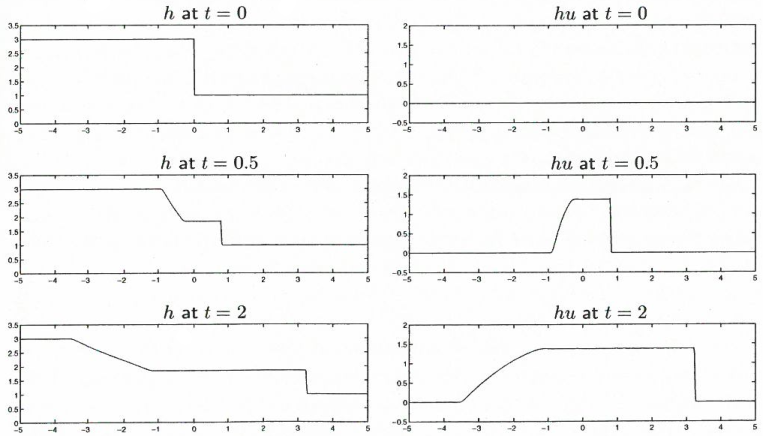
\includegraphics[width=0.75\textwidth]{figs/leveque13p4}
\end{center}

    \begin{itemize}
    \item[$\circ$] nontrivial wave structure with left-going rarefaction and right-going shock
    \end{itemize}
\end{itemize}
\end{frame}


\begin{frame}{Riemann solver options}

\begin{itemize}
\item how should the Riemann solver work?
\item \alert{exact (harder)}:
    \begin{itemize}
    \item[$\circ$] fully-solve the nonlinear Riemann problem
    $$\bq_t + \bbf(\bq)_x = 0, \quad \bq(t_n,x) = \left\{\bQ_L, \bQ_R\right\}$$
    \item[$\circ$] evaluate $\bQ_*$ as the solution $\bq(t,x_*)$ at $x_*=x_{i+1/2}$ for $t>t_n$
    \item[$\circ$] get $\bF_{i+1/2} = \bbf(\bQ_*)$
    \end{itemize}
\item \alert{average-and-linearization (easier)}:
    \begin{itemize}
    \item[$\circ$] compute $\bQ_0$ as an average of $\bQ_L$ and $\bQ_R$
    \item[$\circ$] let $\hat A = \bbf'(\bQ_0)$
    \item[$\circ$] solve Riemann problem for linear system
    $$\bq_t + \hat A \bq_x = 0, \quad \bq(t_n,x) = \left\{\bQ_L, \bQ_R\right\}$$

        \begin{itemize}
        \item use the Riemann invariants $v_k(t,x) = \bw_k^\top \bq(t,x)$ from $\bw_k^\top \hat A = \lambda_k \bw_k^\top$
        \end{itemize}
    \item[$\circ$] evaluate $\bQ_*$ as the solution $\bq(t,x_*)$ at $x_*=x_{i+1/2}$ for $t>t_n$
    \item[$\circ$] get $\bF_{i+1/2} = \bbf(\bQ_*)$
    \end{itemize}
\end{itemize}
\end{frame}


\begin{frame}{Roe approximate solver}

\begin{itemize}
\item for the easier average-and-linearization route, almost all steps are the same as for a linear system (e.g.~acoustics)
\item but how to ``compute $\bQ_0$ as an average of $\bQ_L$ and $\bQ_R$''?
    \begin{itemize}
    \item[1.] low-accuracy approximation results from a simple average:
        $$\bQ_0 = \frac{1}{2} \left(\bQ_L + \bQ_R\right) \implies \hat A = \bbf'(\bQ_0)$$
    \item[2.] different low-accuracy approximation from:
        $$\hat A = \frac{1}{2} \left(\bbf'(\bQ_L) + \bbf'(\bQ_R)\right)$$

        \begin{itemize}
        \item not a good idea; no guarantee $\hat A$ is hyperbolic
        \end{itemize}
    \item[3.] higher-accuracy idea of Roe (1981), called \emph{Roe averaging}:
        $$\begin{matrix} \hat h = \frac{1}{2} (h_L + h_R) {\Large\strut} \\
\hat u = \frac{\sqrt{h_L}\, u_L + \sqrt{h_R}\, u_R}{\sqrt{h_L} + \sqrt{h_R}}
\end{matrix}
\implies \bQ_0 = \begin{bmatrix} \hat h \\ \hat h \hat u \end{bmatrix} \implies \hat A = \bbf'(\bQ_0)$$
    \end{itemize}
\end{itemize}
\end{frame}


\begin{frame}{shallow water: my results}

\begin{itemize}
\item put together the above tools \dots
\item if you do it in C and PETSc and you use PETSc' ODE solvers then \dots you get my program \texttt{riemann} at
    \begin{center}
    \href{https://github.com/bueler/p4pdes-next}{\texttt{github.com/bueler/p4pdes-next}}
    \end{center}
\item if you do it in \Matlab and you use \texttt{ode23} then \dots you get Denys Dutykh's program
\end{itemize}

\vspace{10mm}
\begin{center}
\alert{SHOW SHALLOW WATER ``DAM'' MOVIE}

\bigskip
\alert{SHOW SHALLOW WATER ``HUMP'' MOVIE}
\end{center}
\end{frame}


\begin{frame}{summary}

\begin{itemize}
\item for hyperbolic conservation-law systems $\bq_t + \bbf(\bq)_x = \bg$
    \begin{itemize}
    \item[$\circ$] linear examples $\bbf(\bq)=A\bq$: acoustics, elasticity, Maxwell's equations
    \item[$\circ$] nonlinear examples: shallow water, compressible gas
    \end{itemize}
a preferred numerical approach since the 1990s is a
\begin{center}
\alert{high-resolution Godunov method}
\end{center}
\item consists of three things:
    \begin{itemize}
    \item[\alert{1.}] \alert{finite volume thinking}
        \begin{itemize}
        \item conservation law is spatially integrated
        \item discrete unknowns $\bQ_i$ are cell averages
        \item flux is needed at faces between cells: $\bF_{i+1/2}$
        \end{itemize}
    \item[\alert{2.}] \alert{Riemann solvers}
        \begin{itemize}
        \item the ``Riemann problem'' considers different cell values on each side of a face
        \item a Riemann solver determines the local wave structure (rarefaction, shock)
            \begin{description}[abc]
            \item[$\diamond$] provided by the user; exact or approximate (e.g.~Roe)
            \item[$\diamond$] for a system, uses eigen-expansion of $A = \bbf'(\bq)$
            \item[$\diamond$] compute the flux on the face forward in time
            \end{description}
        \end{itemize}
    \item[\alert{3.}] \alert{slope (or flux) limiters}
        \begin{itemize}
        \item based on first-order upwinding ($=$ donor-cell $=$ ``classical Godunov'')
        \item to achieve higher-order without oscillations:
            \begin{description}[abc]
            \item[$\diamond$] solution is ``reconstructed'' with slope in each cell
            \item[$\diamond$] slope is (nonlinearly) limited
            \item[$\diamond$] the method reverts to first-order upwinding at extrema
            \end{description}
        \end{itemize}
    \end{itemize}
\end{itemize}
\end{frame}


\section{advection again, but 2D spatial}

\begin{frame}{scalar conservation laws in 2D}

\begin{itemize}
\item for this section, the problem is a scalar conservation law in 2D:
    $$q_t + \Div \bF(q) = 0$$

    \begin{itemize}
    \item[$\circ$] the solution is a scalar $q(t,x,y)$ but the flux is a vector $\bF(q)$
    \item[$\circ$] $q$ might be a (conserved) density like mass or energy
    \item[$\circ$] \emph{advection} is when $\bF(q) = \ba q$, where $\ba(x,y) = \left<u(x,y), v(x,y)\right>$ is velocity:
    $$q_t + (u q)_x + (v q)_y = 0$$
    \end{itemize}
\item we want the solution in a region $\Omega\subset \RR^2$, for some times $0\le t \le T$
\end{itemize}
\end{frame}


\begin{frame}{finite volumes in 2D}

\begin{itemize}
\item how does the finite volumes (FV) method work in 2D?
    \begin{itemize}
    \item[$\circ$] the domain on which you solve the PDE is cut into finitely-many cells
	    \begin{itemize}
	    \item[$\diamond$] 1D cells are just intervals
	    \item[$\diamond$] 2D cells are polygons (e.g.~triangles or rectangles, etc.)
	    \item[$\diamond$] 3D cells are polyhedra (e.g.~tetrahedra or cubes, etc.)
	    \end{itemize}
    \item[$\circ$] the method enforces the integrated version of conservation on the cell
    \item[$\circ$] there is one unknown and one equation per cell
    \end{itemize}
\end{itemize}
\end{frame}


\begin{frame}{scalar conservation laws in 2D: integral form}

\begin{itemize}
\item the FV method always starts with the same manipulations \dots
\item suppose $V \subset \RR^2$ is a \emph{finite volume} (cell) in the $x,y$ plane
    \begin{itemize}
    \item[$\circ$] the cell has volume (area) $|V|$
    \end{itemize}
\item integrate the conservation law over the cell:
    $$\int_V q_t\,dx dy + \int_V \Div \bF(q)\,dx dy = 0$$
\item let $Q_V(t)$ be the average of the solution over the cell:
    $$Q_V(t) := \frac{1}{|V|} \int_V q(t,x,y)\,dx dy$$
\item apply divergence theorem:
    $$\frac{dQ_V}{dt} + \frac{1}{|V|} \int_{\partial V} \bF\cdot \bn\,ds = 0$$

    \begin{itemize}
    \item[$\circ$] $\partial V = \text{boundary of } V$
    \end{itemize}
\end{itemize}
\end{frame}


\begin{frame}{structured finite volumes in 2D}

\begin{itemize}
\item PDE $q_t + \Div \bF(q) = 0$ has become an ODE for $Q_V$:
    $$\frac{dQ_V}{dt} + \frac{1}{|V|} \int_{\partial V} \bF\cdot \bn\,ds = 0$$
\item suppose region $\Omega$ is a rectangle: \quad $\Omega = [a,b] \times [c,d]$
\item a \emph{structured} FV method cuts $\Omega$ into a grid of indexed cells $V_{ij}$
    \begin{itemize}
    \item[$\circ$] rectangular cells have dimensions $h_x,h_y$ and area $|V_{ij}| = h_x h_y$
    \end{itemize}
\item apply the equation for each cell:
    $$\frac{dQ_{ij}}{dt} + \frac{1}{h_x h_y} \int_{\partial V_{ij}} \bF\cdot \bn\,ds = 0 \hspace{50mm}$$
\item get a system of ODEs: $\ds \frac{d\bQ}{dt} = \bG(t,\bQ)$
\item to actually construct $\bG$ for this system

we need a method for computing the

flux $\bF$ on the boundary of each $V_{ij}$
\end{itemize}

\vspace{-40mm}
\hfill 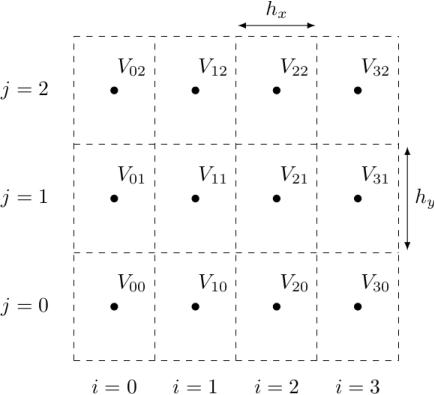
\includegraphics[width=0.35\textwidth]{figs/bueler11p1}
\end{frame}


\begin{frame}{advection in 2D}

\begin{itemize}
\item consider advection with $\bF(q) = \ba q$ where $\ba = \left<u,v\right>$:
\begin{align*}
\frac{dQ_{ij}}{dt} + \frac{1}{h_x h_y} \int_{\partial V_{ij}} \left<uq,vq\right> \cdot \bn \,ds &= 0
\end{align*}
\item the boundary $\partial V_{ij}$ has 4 sides (faces) $N,E,S,W$
\item thus need 4 integrals:
    $$\int_{\partial V_{ij}} \left<uq,vq\right> \cdot \bn \,ds = \int_N + \int_E + \int_S + \int_W \hspace{50mm}$$

    \begin{itemize}
    \item[$\circ$] actually, only compute $N,E$ faces \dots
    \end{itemize}

\item simplest integral (\emph{quadrature}) choice uses

the value at the midpoint of the face

    \begin{itemize}
    \item[$\circ$] open circles in figure
    \end{itemize}
\end{itemize}

\vspace{-35mm}
\hfill 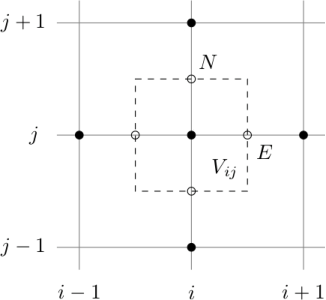
\includegraphics[width=0.33\textwidth]{figs/bueler11p8facemidpoints}
\end{frame}


\begin{frame}{upwinding (donor-cell) in 2D}

\begin{itemize}
\item consider advection with $\bF(q) = \ba q$ where $\ba = \left<u,v\right>$
\item the simplest (Godunov) ``donor cell'' upwinding method decides which side contributes the solution value $Q$ when computing the flux
\item for example, at $N = (x_i,y_j+\tfrac{h_y}{2})$ the normal direction is $\hat \by = \left<0,1\right>$:
\begin{align*}
\int_N \left<uq,vq\right> \cdot \bn \,ds &= \int_N \left<uq,vq\right> \cdot \left<0,1\right> \,ds \\
   &= \int_N vq \,ds \\
   &\approx h_x\, v(N) \tilde Q  \quad [\text{\footnotesize midpoint rule}] \hspace{40mm}
\end{align*}

where
    $$\tilde Q = \begin{cases} Q_{i,j}   & v(N) \ge 0 \\
                               Q_{i,j+1} & v(N) < 0 \end{cases} \hspace{40mm}$$
\item such decisions are made at all 4 faces

    \begin{itemize}
    \item[$\circ$] figure: at $N$ and $E$ faces for given $\ba$
    \end{itemize}
\end{itemize}

\vspace{-45mm}
\hfill 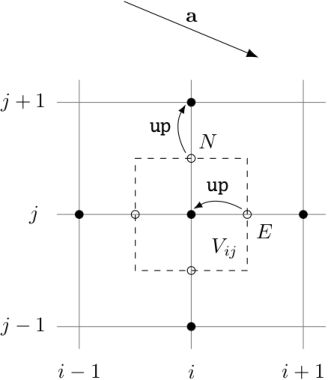
\includegraphics[width=0.33\textwidth]{figs/bueler11p8upwind}
\end{frame}


\begin{frame}{higher-resolution schemes in 2D}

\begin{itemize}
\item recall that the Riemann problem has an initial condition of two values $Q_L$, $Q_R$ on the sides of a face
\item important principle for 2D and 3D FV schemes:

\bigskip
\hfill \alert{the Riemann problem on each face is treated as 1D, normal to the face}

\bigskip
    \begin{itemize}
    \item[$\circ$] e.g.~for advection, first-order upwinding looks only at the component of velocity normal to the face
    \end{itemize}
\item two flavors of ``high-resolution'' schemes:
    \begin{enumerate}
    \item \emph{slope limiters} regard the solution in each cell as not constant, and then modify the slopes to avoid oscillations
    \item \emph{flux limiters} compute the flux based on first-order upwinding, with an added term based on a higher-order flux, but limited to avoid oscillations
    \end{enumerate}
    \begin{itemize}
    \item[$\circ$] these 2 modern routes are (essentially) equivalent in 1D
    \item[$\circ$] flux limiters may be more natural in 2D and 3D?
    \end{itemize}
\end{itemize}
\end{frame}


\begin{frame}{a flux-limiter scheme}

\begin{itemize}
\item recall that at the $N$ face of cell $V_{ij}$, first-order (donor-cell) upwinding was
    $$\int_N \left<uq,vq\right> \cdot \bn \,ds \approx h_x\, \alert{v(N) \tilde Q} \quad \text{where} \quad \tilde Q = \begin{cases} Q_{i,j}   & v(N) \ge 0 \\
                               Q_{i,j+1} & v(N) < 0 \end{cases}$$
\item normal flux at the center of $N$ face is: \quad $f_N = v(N) \tilde Q$
\item with a flux-limiter $\psi$ we instead have
    $$f_N = v(N) \begin{cases} Q_{i,j} + \psi(\theta_j) (Q_{i,j+1}-Q_{i,j})   & v(N) \ge 0 \\
                               Q_{i,j+1} + \psi(1/\theta_{j+1}) (Q_{i,j}-Q_{i,j+1}) \hspace{5mm} & v(N) < 0 \end{cases}$$
where $\ds \theta_j = \frac{Q_{i,j}-Q_{i,j-1}}{Q_{i,j+1}-Q_{i,j}}$

\small
\item $\psi(\theta)$ is a curve in the famous

Sweby (1984) shaded region
    \begin{itemize}
    \item[$\circ$] solid: van Leer (1974)
    \item[$\circ$] dashed: Koren (1993)
    \end{itemize}
\end{itemize}

\vspace{-26mm}
\hfill 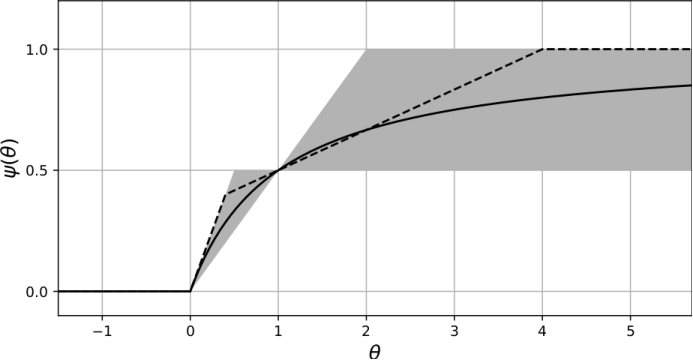
\includegraphics[width=0.45\textwidth]{figs/bueler11p6}
\end{frame}


\begin{frame}{flux-limiters in 2D: decision schematic}

\begin{itemize}
\item make decisions at $N,E$ faces \dots this suffices
\item compare: first-order upwinding (left) versus the flux-limiter case (right) using ``downwind'' (\textbf{\texttt{dn}}) and ``far'' points (\textbf{\texttt{far}})
    \begin{itemize}
    \item[$\circ$] a flux- or slope-limiter is \emph{stencil expanding}
    \end{itemize}
\end{itemize}

\bigskip
\quad \mbox{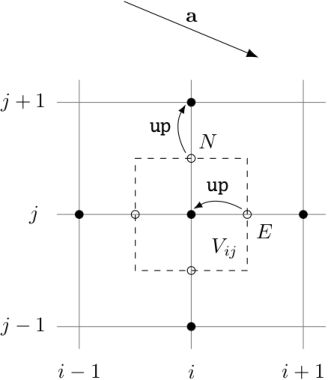
\includegraphics[width=0.34\textwidth]{figs/bueler11p8upwind} \hspace{15mm} 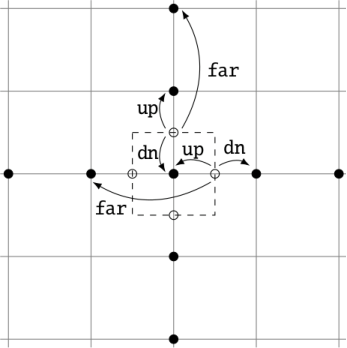
\includegraphics[width=0.38\textwidth]{figs/bueler11p8fluxlimited}}
\end{frame}


\begin{frame}{results}

\begin{itemize}
\item suppose domain is square $\Omega = (-1,1) \times (-1,1)$ and equation $q_t + \Div \bF(q) = 0$ is advection ($\bF(q) = \ba q$) with a rotation velocity field:
    $$\ba(x,y) = \left<y,-x\right>$$
\item solving for $0\le t \le 2\pi$ should rotate initial condition back to itself
\item results on a $40\times 40$ grid with the Koren flux limiter and an adaptive, 2nd-order Runge-Kutta ODE solver ($\approx$ \texttt{ode23}):

\bigskip
\hfill 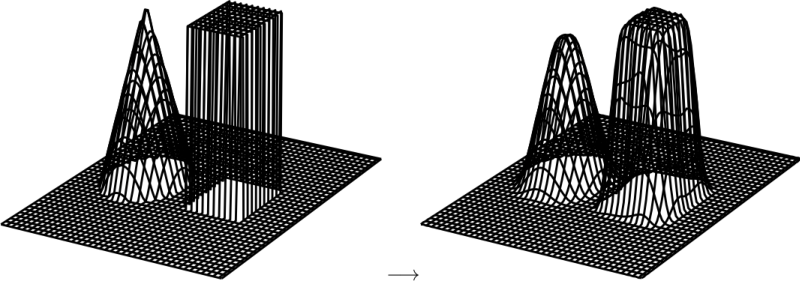
\includegraphics[width=0.75\textwidth]{figs/bueler11p7}

\medskip
    \begin{itemize}
    \item[$\circ$] good results like this would require \emph{much} finer grid using Lax-Wendroff ($1000\times 1000$?)
    \end{itemize}
\end{itemize}
\end{frame}


\begin{frame}[fragile]
\frametitle{live movie, computed in parallel}

\begin{itemize}
\item see \texttt{c/ch11/advect.c} at \href{https://github.com/bueler/p4pdes}{\texttt{github.com/bueler/p4pdes}}
    \begin{itemize}
    \item[$\circ$] uses C and PETSc and MPI
    \end{itemize}
\item runs here use Koren flux-limiter and SSP time-stepping
    \begin{itemize}
    \item[$\circ$] \emph{strong stability-preserving} (SSP) is better than RK
    \end{itemize}
\item movie from parallel run with 4 processors:
\begin{Verbatim}[fontsize=\footnotesize]
$ tmpg -n 4 ./advect -adv_problem rotation \
    -da_refine 3 -ts_max_time 6.283185 \
    -ts_monitor_solution draw \
    -ts_type ssp -adv_limiter koren
\end{Verbatim}
%$

\vspace{-20mm}
\hfill 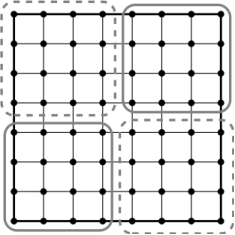
\includegraphics[width=0.22\textwidth]{figs/buelerfourproc}

\vspace{-1mm}
\item parallel run with 12 processes in 90 seconds:
    \begin{itemize}
    \item[$\circ$] $N=640\times 640 \times 4022 = 1.6 \times 10^9$ \dots billion-point space-time grid
    \end{itemize}
\begin{Verbatim}[fontsize=\footnotesize]
$ tmpg -n 12 ./advect -adv_problem rotation -da_refine 7 \
    -ts_max_time 6.283185 -ts_type ssp -adv_limiter koren \
    -ts_view_solution draw -draw_pause -1
\end{Verbatim}
%$

\bigskip
\hspace{15mm} \alert{SHOW}
\end{itemize}
\end{frame}

\end{document}

